\documentclass[a4paper,11pt,oneside]{book}
\usepackage{listings}
\usepackage[utf8]{inputenc}
\usepackage[spanish]{babel}
\usepackage{float}
\usepackage{enumitem} % Para listas con mejor control

\usepackage{changepage}





% Configura la profundidad de numeración hasta subsubsecciones
\setcounter{secnumdepth}{3}


\decimalpoint
\usepackage{dcolumn}
\newcolumntype{.}{D{.}{\esperiod}{-1}}
\makeatletter
\addto\shorthandsspanish{\let\esperiod\es@period@code}
\makeatother

\RequirePackage{verbatim}
\usepackage{fancyhdr}
\usepackage{graphicx}
\usepackage{afterpage}

\usepackage{longtable}

\usepackage[pdfborder={0 0 0}]{hyperref} % referencia


% ********************************************************************
% Re-usable information
% ********************************************************************
\newcommand{\myTitle}{Aplicación para la gestión de una tienda minorista\xspace}
\newcommand{\myDegree}{Grado en Ingeniería Informática\xspace}
\newcommand{\myName}{Julia María Cano Flores \xspace}
\newcommand{\myProf}{María Luisa Rodríguez Almendros \xspace}
\newcommand{\myFaculty}{Escuela Técnica Superior de Ingenierías Informática y de Telecomunicación\xspace}
\newcommand{\myFacultyShort}{E.T.S. de Ingenierías Informática y de Telecomunicación\xspace}
\newcommand{\myDepartment}{Departamento de Lenguajes y Sistemas Informáticos\xspace}
\newcommand{\myUni}{\protect{Universidad de Granada}\xspace}
\newcommand{\myLocation}{Granada\xspace}
\newcommand{\myTime}{\today\xspace}
\newcommand{\myVersion}{Version 0.1\xspace}

\hypersetup{
	pdfauthor = {\myName (email (en) ugr (punto) es)},
	pdftitle = {\myTitle},
	pdfsubject = {},
	pdfkeywords = {palabra_clave1, palabra_clave2, palabra_clave3, ...},
	pdfcreator = {LaTeX con el paquete ....},
	pdfproducer = {pdflatex}
}

\usepackage{url}
\usepackage{colortbl,longtable}
\usepackage[stable]{footmisc}
\usepackage{index}

\usepackage{tabularx} 
\usepackage{pdflscape}  % Controlar la página en horizontal.


\makeindex


\pagestyle{fancy}
\fancyhf{}
\fancyhead[LO]{\leftmark}
\fancyhead[RE]{\rightmark}
\fancyhead[RO,LE]{\textbf{\thepage}}
\renewcommand{\chaptermark}[1]{\markboth{\textbf{#1}}{}}
\renewcommand{\sectionmark}[1]{\markright{\textbf{\thesection. #1}}}


\usepackage{fancyhdr}
\pagestyle{fancy}
\fancyhf{} % Limpia el encabezado y pie de página de configuraciones previas
\fancyfoot[C]{\thepage} % Centra el número de página en el pie de página
\renewcommand{\headrulewidth}{0pt} % Elimina la línea del encabezado
\renewcommand{\footrulewidth}{0pt} % Elimina la línea del pie de página si existe

% Corrige cualquier espacio adicional alrededor del área del pie de página que podría desplazar el número de la página
\fancyfootoffset{0pt}


\usepackage{booktabs} % Para obtener líneas horizontales mejoradas
\usepackage[table]{xcolor}

\usepackage{apacite}
\bibliographystyle{apacite}


\setlength{\headheight}{1.5\headheight}

% Configuraciones de colores y listados

\begin{document}
	% Portada
	\begin{titlepage}
 
 
\newlength{\centeroffset}
\setlength{\centeroffset}{-0.5\oddsidemargin}
\addtolength{\centeroffset}{0.5\evensidemargin}
\thispagestyle{empty}

\noindent\hspace*{\centeroffset}\begin{minipage}{\textwidth}

\centering

\includegraphics[width=0.9\textwidth]{imagenes/logo_ugr.jpg}\\[1.4cm]

\textsc{ \Large TRABAJO FIN DE GRADO\\[0.2cm]}
\textsc{ INGENIERÍA INFORMÁTICA}\\[1cm]
% Upper part of the page
% 
% Title
{\Huge\bfseries Aplicación para la gestión de una tienda minorista\\
}
\noindent\rule[-1ex]{\textwidth}{3pt}\\[3.5ex]

\end{minipage}

\vspace{2.5cm}
\noindent\hspace*{\centeroffset}\begin{minipage}{\textwidth}
\centering

\textbf{Autor}\\ {Julia María Cano Flores}\\[2.5ex]
\textbf{Directores}\\
{María Luisa Rodríguez Almendros}\\[2cm]

\includegraphics[width=0.3\textwidth]{imagenes/etsiit_logo.png}\\[0.1cm]
\textsc{Escuela Técnica Superior de Ingenierías Informática y de Telecomunicación}\\
\textsc{---}\\
Granada, febrero de 2024
\end{minipage}
%\addtolength{\textwidth}{\centeroffset}
%\vspace{\stretch{2}}
\end{titlepage}
\clearpage



	% Suprime la numeración de esta página
	\thispagestyle{empty}
	% Asegura que la numeración comience en la siguiente página
	\clearpage
	\setcounter{page}{2}
	
	% Prefacios y otros elementos preliminares
	\begin{titlepage}
 
 
\setlength{\centeroffset}{-0.5\oddsidemargin}
\addtolength{\centeroffset}{0.5\evensidemargin}
\thispagestyle{empty}

\noindent\hspace*{\centeroffset}\begin{minipage}{\textwidth}

\centering
%
\includegraphics[width=0.9\textwidth]{imagenes/logo_ugr.jpg}\\[1.4cm]

%\textsc{ \Large PROYECTO FIN DE CARRERA\\[0.2cm]}
%\textsc{ INGENIERÍA EN INFORMÁTICA}\\[1cm]
% Upper part of the page
% 

 \vspace{3.3cm}

%si el proyecto tiene logo poner aquí

\includegraphics{imagenes/logo.png} 
 \vspace{0.5cm}

% Title

{\Huge\bfseries Aplicación para la gestión de una tienda minorista\\
}
\noindent\rule[-1ex]{\textwidth}{3pt}\\[3.5ex]

\end{minipage}

\vspace{2.5cm}
\noindent\hspace*{\centeroffset}\begin{minipage}{\textwidth}
\centering

\textbf{Autor}\\ {Julia María Cano Flores}\\[2.5ex]
\textbf{Directores}\\
{María Luisa Rodríguez Almendros}\\[2cm]

\includegraphics[width=0.15\textwidth]{imagenes/tstc.png}\\[0.1cm]
\textsc{Departamento de Lenguajes y Sistemas Informáticos}\\
\textsc{---}\\
Granada, febrero de 2024
\end{minipage}
\addtolength{\textwidth}{\centeroffset}
\vspace{\stretch{2}}

 
\end{titlepage}





\cleardoublepage
%\thispagestyle{empty}

\begin{center}
{\large\bfseries Aplicación para la gestión de una tienda minorista}\\
\end{center}
\begin{center}
Julia María Cano Flores\\
\end{center}

\vspace{0.7cm}
\noindent{\textbf{Palabras clave}: minorista, base de datos, software, requisitos}\\

\vspace{0.7cm}
\noindent{\textbf{Resumen}}\\

El desarrollo de este Trabajo Fin de Grado (TFG) tiene como finalidad principal simplificar y mejorar la eficiencia de la gestión de negocios minoristas. Está diseñado para optimizar el proceso de seguimiento de ventas mediante una base de datos que registre todas las transacciones realizadas. El sistema no solo registra compras y devoluciones, sino que también incorpora una característica distintiva: la gestión de préstamos. Esta funcionalidad es particularmente útil en localidades pequeñas, donde las relaciones de confianza entre comerciantes y clientes permiten prácticas como llevarse productos sin un desembolso inicial. Los clientes pueden probar los artículos antes de comprometerse a la compra o optar por la devolución sin costos adicionales.\\


El software proporcionará una interfaz de usuario intuitiva compuesta de múltiples pantallas, entre las que podemos destacar un inventario actualizado en tiempo real, la visualización de los artículos en venta o una lista de clientes habituales del negocio. Además, para impulsar la toma de buenas decisiones estratégicas, el programa generará gráficos analíticos que reflejarán el progreso económico del negocio. \\

Este proyecto surge de la necesidad evidente de una solución tecnológica adaptada a los requisitos específicos de los negocios minoristas. Hasta el momento, son negocios que no se han tenido en cuenta debido a su bajo impacto y su pequeño tamaño. Sin embargo, debemos de mirar por llevar la tecnología a todos los ámbitos. Esta aplicación busca llenar ese vacío y convertirse en una herramienta útil para comerciantes minoristas.  


\cleardoublepage


%\thispagestyle{empty}


\begin{center}
{\large\bfseries Application for the management of a retail store}\\
\end{center}
\begin{center}
Julia María Cano Flores\\
\end{center}

\vspace{0.7cm}
\noindent{\textbf{Keywords}: retailer, database, software, requirements}\\

\vspace{0.7cm}
\noindent{\textbf{Abstract}}\\


The main purpose of the development of this Final Degree Project (FDP) is to simplify and improve the efficiency of retail business management. It is designed to optimize the sales tracking process through a database that records all transactions made. The system not only records purchases and returns but also incorporates a distinctive feature: loan management. This functionality is particularly useful in small localities, where trust relationships between merchants and customers allow practices such as taking products without an initial outlay. Customers can test items before committing to purchase or opt for a return without additional costs.\\

The software will provide an intuitive user interface composed of multiple screens, among which we can highlight an inventory updated in real-time, the display of items for sale, or a list of regular customers of the business. In addition, to drive good strategic decision-making, the program will generate analytical charts that will reflect the economic progress of the business.\\

This project arises from the clear need for a technological solution adapted to the specific requirements of retail businesses. So far, they are businesses that have not been considered due to their low impact and small size. However, we must look to bring technology to all areas. This application seeks to fill that void and become a useful tool for retail merchants.



\chapter*{}

%\thispagestyle{empty}


\noindent\rule[-1ex]{\textwidth}{2pt}\\[4.5ex]

Yo, \textbf{Julia María Cano Flores}, alumna de la titulación INGENIERÍA INFORMÁTICA de la \textbf{Escuela Técnica Superior
de Ingenierías Informática y de Telecomunicación de la Universidad de Granada}, con DNI 77649643x, autorizo la
ubicación de la siguiente copia de mi Trabajo Fin de Grado en la biblioteca del centro para que pueda ser
consultada por las personas que lo deseen.

\vspace{6cm}

\noindent Fdo: Julia María Cano Flores

\vspace{2cm}

\begin{flushright}
Granada a 2 de febrero de 2024 .
\end{flushright}


\chapter*{}
%\thispagestyle{empty}

\noindent\rule[-1ex]{\textwidth}{2pt}\\[4.5ex]

D. \textbf{María Luisa Rodríguez Almendros}, Profesora del Área de Ingeniería del Software del Departamento de Lenguajes y Sistemas Informáticos de la Universidad de Granada.




\vspace{0.5cm}

\textbf{Informan:}

\vspace{0.5cm}

Que el presente trabajo, titulado \textit{\textbf{Aplicación para la gestión de una tienda minorista}},
ha sido realizado bajo su supervisión por \textbf{Julia María Cano Flores}, y autorizamos la defensa de dicho trabajo ante el tribunal
que corresponda.

\vspace{0.5cm}

Y para que conste, expiden y firman el presente informe en Granada a 2 de febrero de 2024 .

\vspace{1cm}

\textbf{Los directores:}

\vspace{5cm}

\noindent \textbf{María Luisa Rodríguez Almendros}

\chapter*{Agradecimientos}
\thispagestyle{empty}

       \vspace{1cm}


Poner aquí agradecimientos...




	
	\tableofcontents
	\listoffigures
	\listoftables
	
%	\mainmatter
	\setlength{\parskip}{5pt}
	
	% Contenido principal
	\chapter{Introducción}
\label{chap:introduction}

\section{Motivación}
\label{sec:motivation}

Se entiende como negocio minorista toda empresa de comercio que adquiere mercancías por cuenta propia, y las revende directamente al consumidor final. En negocios minoristas pequeños podemos encontrar un trato más cercano con los clientes y una forma algo distinta de gestionar un comercio. \\

Al ser nacida y criada en un pueblo, la mayoría de negocios con los que he crecido eran comercios minoristas pequeños. Además, mi padre es propietario de una tienda y he podido conocer de primera mano cuál es el funcionamiento real de este tipo de negocios. Tras una vida tratando con ellos y una entrevista realizada a mi padre, he encontrado la necesidad de informatizar este trabajo con el objetivo de conseguir optimizar el rendimiento y llevar un seguimiento. En la actualidad, muchos comerciantes minoristas no disponen de grandes tecnologías y recurren a métodos tradicionales basados en papel para el seguimiento de su negocio. Esto tiene un riesgo alto de pérdida de datos o cometer errores. 
Además, el proceso de recuperación y análisis de datos se convierten en tareas muy tediosas, ya que la falta de sistemas automatizados impide un filtrado eficiente de información. Todo esto ralentiza el trabajo de forma significativa, haciendo que la productividad del comerciante sea menor y, por tanto, la evolución del negocio no sea óptima. \\

En el mercado actual no encontramos aplicaciones que pongan solución al problema de los negocios minoristas pequeños. Las soluciones software existentes tienden a enfocarse en entidades de mayor escala. Como hemos visto, los negocios minoristas tienen singularidades que conllevan establecer requisitos específicos y tratar su gestión de forma independiente a la gestión de un gran negocio. Por ello, es crucial el desarrollo de un software que satisfaga las necesidades de los pequeños comerciantes y les permita conducir su negocio a una evolución óptima. 


\section{Objetivos del proyecto}
\label{sec:project_objectives}

El objetivo general de este proyecto es proporcionar una solución informática analizando los procedimientos típicos de un comercio minorista pequeño que actualmente se realizan de forma manual y desarrollando una aplicación que los automatice. Para conseguir dicho objetivo, podemos diferenciar una serie de objetivos específicos: 


% Tabla para el Objetivo 1
\definecolor{grayshade}{gray}{0.9}



\begin{itemize}
	\item \textbf{Objetivo 1: Análisis de los comercios minoristas}
	\begin{itemize}
		\item \textbf{Descripción:} Se debe de realizar una búsqueda de información sobre los negocios minoristas con el objetivo de entender mejor cuáles son sus características.
	\end{itemize}
	
	\item \textbf{Objetivo 2: Estudio de aplicaciones similares}
	\begin{itemize}
		\item \textbf{Descripción:} Análisis del mercado actual de aplicaciones similares para identificar funcionalidades innovadoras que implementar en nuestra aplicación.
	\end{itemize}
	
	\item \textbf{Objetivo 3: Análisis de usabilidad y accesibilidad}
	\begin{itemize}
		\item \textbf{Descripción:} Estudiar soluciones accesibles para conseguir una aplicación fácil de usar para la mayoría de usuarios.
	\end{itemize}
	
	\item \textbf{Objetivo 4: Análisis de las tecnologías a utilizar}
	\begin{itemize}
		\item \textbf{Descripción:} Investigar sobre cuáles son las mejores tecnologías para llevar a cabo el proyecto.
	\end{itemize}
	
	\item \textbf{Objetivo 5: Desarrollo e implementación de la aplicación}
	\begin{itemize}
		\item \textbf{Descripción:} Analizar, desarrollar y probar la aplicación con el objetivo de conseguir los mejores resultados.
	\end{itemize}
	
	\item \textbf{Objetivo 6: Validación de la aplicación por usuarios reales}
	\begin{itemize}
		\item \textbf{Descripción:} Poner a prueba la aplicación en un entorno real para ver si cumple las expectativas del usuario.
	\end{itemize}
\end{itemize}

\section{Estructura del documento}
\label{sec:document_structure}
Esta sección se ofrece una visión de la estructura y organización del documento. Se compone de las siguientes partes: 

\begin{itemize}
	\item \textbf{Resumen:} Un resumen donde se exponen las principales funcionalidades del proyecto y sus objetivos. 
	
	\item \textbf{Introducción:} En este apartado se exponen los principales objetivos que se pretenden cumplir durante el desarrollo del proyecto. Además, se explica la motivación por la que se empezó a idear dicho proyecto a modo de introducción. 

	
	\item \textbf{Planificación:} Especificación de la planificación del proyecto, donde se muestran las distintas fases y la estimación presupuestaria del mismo. 
	
	\item \textbf{Estado del arte:} Investigación sobre los principales temas que se tratan en el proyecto como los negocios minoristas, los negocios mixtos y los comerciantes minoristas. Además, se tratan temas legales como la protección de datos. Con esta investigación, entramos en contexto para posteriormente entender los requisitos del proyecto. 
	
	\item \textbf{Análisis de tecnologías a utilizar:} Enumeración de tecnologías utilizadas para el desarrollo del proyecto. Para cada tecnología, se explica porqué se ha utilizado y se citan sus principales características. 
	
	\item \textbf{Análisis de la aplicación:} Obtención y explicación de los requisitos del sistema. Posteriormente se amplia esta información desarrollando los casos de uso, el modelo conceptual y los diagramas de secuencia del sistema. 
	
	\item \textbf{Diseño:} Descripción de la arquitectura del sistema, el diseño de las clases necesarias para el programa y la interfaz de usuario.
	
	\item \textbf{Implementación de la aplicación:} La implementación de la aplicación se desarrollará en con una metodología ágil, por lo que este capítulo se dividirá en sus iteraciones. 
	
	\item \textbf{Bibliografía:} Recopilación de todas las fuentes de información utilizadas durante la realización del proyecto.
\end{itemize}
\newpage






	
	\chapter{Planificación}
\label{chap:planification}


\section{Fases}

La planificación del desarrollo del proyecto se ha dividido en las fases que vamos a ver a continuación.

\subsection{Fase inicial}

En esta etapa es donde se definen las bases del proyecto. Se expone la motivación que nos conduce a llevar el proyecto a cabo, se identifican las necesidades y se establecen unos objetivos principales que deberán de cumplirse a lo largo del desarrollo del proyecto. Esta información podemos verla en el capítulo 1 (\hyperref[chap:introduction]{ver página}) de este documento. 

\subsection{Fase de investigación}

Durante esta fase, se recopila información para entender el entorno donde se pondrá en práctica la aplicación. Para ello, se investigarán cuestiones como la definición de negocio minorista, un estudio de los pequeños negocios mixtos y un estudio de los comerciantes minoristas. Además, con el objetivo de que la aplicación cumpla los términos legales, también se realizará un estudio sobre usabilidad, accesibilidad y la legislación de protección de datos. 

Para finalizar esta fase de investigación y entender la verdadera necesidad de desarrollar esta aplicación, se realizará una comparación de aplicaciones similares en el mercado. 

\subsection{Fase de análisis}

En esta fase encontraremos 2 apartados: 

\begin{itemize}
	\item \textbf{Análisis de las tecnologías:} En este apartado encontraremos una lista de las tecnologías que se han utilizado para el desarrollo del proyecto, además de una explicación de porqué han sido seleccionadas y cuáles son sus principales características.  
	\item \textbf{Análisis de la aplicación:} Durante este aparado se estudian los requisitos que deberá de cumplir la aplicación para satisfacer las necesidades del cliente. Para una mayor especificación y claridad, se desarrollarán los casos de uso y los diagramas de secuencia del sistema. Para entender como se relacionan las entidades, también se hará un modelo conceptual. 
\end{itemize}


\subsection{Fase de diseño}

En esta fase, se especifica más en detalle cómo va a construirse la aplicación mediante un diagrama de la arquitectura del sistema y los bocetos de la interfaz gráfica del usuario. Los bocetos se harán pantalla a pantalla y organizados por los mismos grupos que los requisitos para una mayor claridad. 


\subsection{Fase de desarrollo}

Esta es la fase donde se construye el producto que hemos definido en la fase de análisis y diseño. Será la etapa más larga ya que se transforman todos los planes y diseños previos en código, dando como resultado un entregable final funcional.\\

Esta fase se dividirá en tres iteraciones, ya que la metodología utilizada para la implementación de la aplicación es una metodología ágil. En cada iteración se escogerá el alcance de la iteración, es decir, los requisitos que se van a llevar a cabo, se realizará la implementación de estos, se testeará y se le expondrá al usuario para que pueda validarlo. Con la validación de usuario se obtendrá información de mejoras que deberán de ser aplicadas en las siguientes iteraciones. 

Tras finalizar las tres iteraciones, se obtendrá un entregable final funcional que se le proporcionará al cliente para que pueda disfrutar de este. 


\subsection{Redacción de la memoria}

Con el objetivo de documentar el desarrollo del proyecto, se va a plasmar toda la información relevante en este documento. No se ha incluido en ninguna fase ya que la documentación se irá haciendo a lo largo de todo el desarrollo del proyecto. 

\subsection{Diagrama de Gantt}

En la siguiente tabla podemos ver cuál ha sido la duración en horas de cada una de las tareas que se exponen en el diagrama de Gantt. El diagrama representa la planificación temporal de las tareas del proyecto. Cada celda representa una semana del mes. En la tabla se muestran las horas y en el diagrama el momento en el que se realizó. 

\begin{table}[h!]
	\centering
	\begin{tabular}{|l|c|}
		\hline
		\textbf{Fase} & \textbf{Horas} \\ \hline
		Motivación & 2 \\ \hline
		Objetivos del proyecto & 3 \\ \hline
		Estructura del documento & 2 \\ \hline
		Definición de un negocio minorista & 10 \\ \hline
		Estudio de los pequeños negocios mixtos & 10 \\ \hline
		Estudio de comerciantes minoristas & 10 \\ \hline
		Estudio de usabilidad y accesibilidad & 12 \\ \hline
		Legislación actual de protección de datos & 5 \\ \hline
		Aplicaciones similares y comparativas & 15 \\ \hline
		Análisis de tecnologías a utilizar & 10 \\ \hline
		Especificación de requisitos & 15 \\ \hline
		Modelos de casos de uso & 20 \\ \hline
		Modelo conceptual & 3 \\ \hline
		Modelos de comportamiento & 20 \\ \hline
		Diagrama de arquitectura del sistema & 1 \\ \hline
		Diseño de la interfaz gráfica & 10 \\ \hline
		Primera iteración & 40 \\ \hline
		Segunda iteración & 45 \\ \hline
		Tercera iteración & 30 \\ \hline
		Creación y modificaciones de la base de datos & 15 \\ \hline
		Redacción de la memoria & 40 \\ \hline
		\textbf{Total} & \textbf{308} \\ \hline
	\end{tabular}
	\caption{Distribución de horas por fase}
	\label{tabla:resumen}
\end{table}



\newpage

\begin{figure}[H]
	\centering
	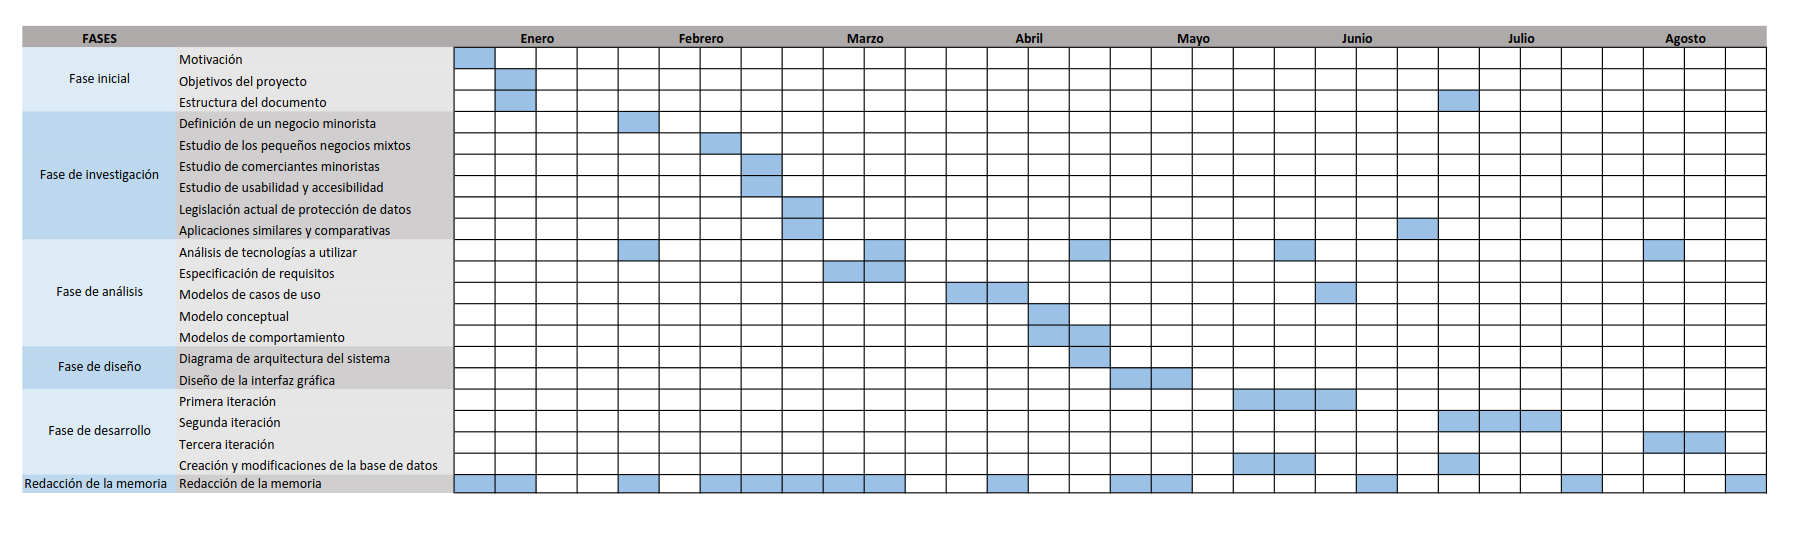
\includegraphics[width=1.6\textwidth, angle=90]{imagenes/imagenesDiagramas/diagramaGantt.png}
	\caption{Diagrama de Gantt}
	\label{fig:diagramaGantt}
\end{figure}



\newpage

\section{Presupuesto}

\subsection{Recursos}

En este apartado se va a exponer los recursos hardware y software que se van a utilizar para el desarrollo del proyecto. 

\begin{adjustwidth}{2em}{0pt} % Aumenta el margen izquierdo por 2em
\subsubsection{Hardware}

Los componentes hardware que se van a utilizar para llevar a cabo el proyecto son: 

\begin{itemize}
	\item \textbf{Ordenador:} MSI Prestige 15 A10SC.
\end{itemize}

\subsubsection{Software}

Las herramientas software que se van a utilizar para llevar a cabo el proyecto son: 

\begin{itemize}
	\item \textbf{Sistema Operativo:} Ubuntu 20.04
	\item \textbf{Lenguaje de programación:} Flutter
	\item \textbf{IDE:} Visual Studio Code
	\item \textbf{Diseño de diagramas UML:} Visual Paradigm
	\item \textbf{Sistema de composición de texto:} LaTeX
	\item \textbf{Editor de texto:} TeXstudio
\end{itemize}
\end{adjustwidth} 

\subsection{Costes}

En esta sección vamos a analizar el coste total del proyecto. Vamos a distinguir distintos apartados. 

\begin{adjustwidth}{2em}{0pt} % Aumenta el margen izquierdo por 2em
	\subsubsection{Licencias}
	
	Un tipo de coste que conlleva el desarrollo de un proyecto es la adquisición de las licencias necesarias para la producción del mismo. Las licencias que se van a utilizar en este proyecto son de software libre y por tanto son gratuitas. Esto significa que no supondrán ningún coste adicional. Las licencias que se utilizarán son las siguientes: 

\newpage

	\begin{itemize}
		\item \textbf{Ubuntu 20.04:} GNU General Public Licence (GPL).
		\item \textbf{Flutter:} Licencia BSD. 
		\item \textbf{Visual Paradigm:} Licencia adquirida por usos académicos. 
		\item \textbf{LaTeX:} LaTeX Project Public License (LPPL).
	\end{itemize}
	
	
	\subsubsection{Recursos materiales}
	
	El único recurso material que se va utilizar para el desarrollo del proyecto es el ordenador personal. \\
	
	El periodo de amortización común para los ordenadores y equipos informáticos es de 3 a 5 años. Realizaremos la media y utilizaremos un periodo de 4 años para los cálculos. Sabiendo que el equipo costó 1400€, se amortizará 350€ al año. Como la duración del proyecto es de 5 meses, el coste final de los recursos materiales será de 145'83€
	
	\subsubsection{Recursos humanos}
	
	En esta sección se incluyen los gastos por la contratación de personal. Este proyecto solamente lo va a desarrollar una persona, bajo la titulación de programador senior. \\
	
	En la actualidad, un programador senior recibe una media de 22.000€ anuales. Durante los 5 meses que dura el proyecto, se estima un salario de 9166'66€. 
	
	\subsubsection{Otros}
	
	Este apartado engloba costes indirectos como los gastos debidos a la localización para trabajar, los gastos de transporte, conexión a Internet, etc. Este gasto se suele aproximar a un 10\% de los gastos de recursos humanos. Por tanto, la cantidad estipulada para este apartado sería de 916'66€. 
	
	\newpage
	
	\subsubsection{Total}
	
% Tabla presupuesto total
\begin{table}[htb!]
	\centering % Centra la tabla en la página
	\begin{tabular}{|p{0.3\linewidth}|p{0.35\linewidth}|p{0.35\linewidth}|}
		\hline
		\rowcolor{grayshade} \textbf{Descripción} & \textbf{Coste mensual} & \textbf{Coste total} \\
		\hline
		\textbf{Licencias} & 0€ & 0€ \\
		\hline
		\textbf{Recursos materiales} & 29'17€ & 145'83€ \\
		\hline
		\textbf{Recursos humanos} & 1833'33€ & 9166'66€ \\
		\hline
		\textbf{Otros} & 183'33€ & 916'66€ \\
		\hline
		\textbf{Total} & 2045,83€ & 10.229'15€ \\
		\hline
	\end{tabular}
	\caption{Presupuesto total}
\end{table}
\end{adjustwidth} 

	
	\chapter{Estado del arte}
\label{chap:EstadoArte}

\section{Definición de un negocio minorista}

La distribución comercial minorista es uno de los sectores de mayor relevancia y dinamismo de nuestra economía. Por tanto, es esencial conocer lo que son, a qué se dedican y cómo se gestionan. \\


Un negocio minorista es una empresa que vende productos o servicios directamente a consumidores finales. Los minoristas actúan como intermediarios entre los fabricantes o mayoristas y el mercado de consumo. Sin los negocios minoristas, los productos fabricados a grande escala nunca llegarían a ser consumidos por los clientes finales. El comerciante ofrece un asesoramiento especializado sobre los productos y servicio de su tienda, así como un trato personalizado. \cite{gestionModerna} \\


Además, el comerciante tiene la responsabilidad de conocer cuál es la cantidad de producto que debe comprar para asegurarse de vender lo máximo posible y conseguir con ello un beneficio económico. En algunas ocasiones, también se encarga de establecer los precios de los productos de su tienda. Para ello, se debe tener en cuenta el precio base del producto y se le añade un porcentaje para cubrir los gastos y conseguir beneficios. La otra posibilidad es que los precios de venta al mercado de consumo estén fijados en el etiquetado por los fabricantes. En ese caso, el comerciante no deberá modificar el precio previamente estimado. \\


Podemos clasificar los negocios minoristas según varios criterios, lo cual nos ayudará a entender los tipos que hay y qué funciones tienen cada uno. \\

\textbf{Clasificación de un negocio minorista según su forma de venta \cite{gestionNegocio}: }

\begin{itemize}
	
	\item \underline{Comercio tradicional}:  La mercancía no está a disposición del comprador. El dependiente deberá de proporcionar los artículos al cliente. Podemos identificar tres elementos en este tipo de comercio: el almacén (donde se almacenan los productos), el mostrador (donde se atiende a los clientes) y el vendedor (la persona encargada de asesorar al cliente en sus decisiones de compra y proporcionar el producto al comprador). Ejemplo: carnicerías, farmacias, mercerías, etc. 
	\item \underline{Comercio de libre servicio}: El consumidor tiene libertad para moverse por el espacio de la tienda y elegir los productos a su gusto. En este tipo de comercio el cliente tiene contacto directo con la mercancía, sin intervención del vendedor.  Ejemplos: supermercados, autoservicios, etc. 
	\item \underline{Comercio mixto}: Combina los dos tipos anteriores. El cliente tiene a su disposición la mercancía de la tienda y además el vendedor asesora al comprador sobre sus decisiones dentro de la tienda. Ejemplos: librerías, grandes almacenes, etc. 
	\item \underline{Venta sin establecimiento comercial}: 
	\begin{itemize}
		\item Venta automática: El comprador selecciona un artículo, lo paga y lo recibe en el momento. Ejemplo: Máquina exprendedora. 
		\item Venta ambulante: Se realiza en rastros o mercadillos.
		\item Venta a distancia: El comprador adquiere el producto o servicio a través de un medio de comunicación. Ejemplo: Venta por teléfono, venta por Internet, etc. 
	\end{itemize}
\end{itemize}

\textbf{Clasificación de un negocio minorista según su agregación \cite{wikiMinorista}:}

\begin{itemize}
\item \underline{Comercio independiente o pequeño comercio}: Se trata de la tradicional tienda de barrio caracterizada por sus pequeñas dimensiones y por su sistema de venta a través de un mostrador. Funciona de forma autónoma, independiente de otros comercios de su gremio o zona. 
\item \underline{Comercio asociado o comercio integrado}: Son tiendas que se localizan en el mismo local, como los pequeños establecimientos de alimentación que se agrupan en mercados. Los centros comerciales surgen del desarrollo de estas pequeñas asociaciones. 
\item \underline{Gran distribución}: Grandes empresas que actúan al mismo tiempo como mayoristas y minoristas. Generalmente, son grandes multinacionales. EN este tipo se encuentran los hipermercados, con las marcas blancas.
\item \underline{Franquicia}: Tiendas que forman parte de una cadena. Tienen el mismo nombre e imagen y venden productos similares en diferentes ubicaciones. 
\end{itemize}


Con esta clasificación, hemos podido ver que los negocios minoristas recogen un amplio rango de negocios de distinta escala y distinta gestión interna. En concreto, nos centraremos en el estudio de los pequeños comercios mixtos. Entraremos en más detalle en el próximo punto. 


\section{Estudio de los pequeños negocios mixtos}

Estos pequeños negocios se caracterizan por el asesoramiento acerca de los productos o servicios que disponen. Uno de los motivos por lo que los consumidores escogen este tipo de tiendas es este, porque les permite tomar una mejor decisión en sus compras. Además, suelen ser negocios menos masificados donde la relación con el cliente toma importancia. \cite{gestionNegocio} \\

Con respecto a la variedad de productos que ofrece un pequeño negocio, es esencial que se especialice y se eliminen los artículos que no sean rentables, así como que se adapte a las características y demandas de sus clientes. Hoy en día, existe una gran competencia con las grandes superficies y la compra online. El comerciante debe ser consciente de esa amenaza y debe ser capaz de distinguirse de las grandes empresas ofreciendo a los clientes unos servicios que no puedan encontrar en otros establecimientos. \\

Los pequeños negocios desarrollan sus propias técnicas de promoción para incentivar y fidelizar clientes. Es su forma de combatir la fuerte competencia entre los negocios y marcas. Estas técnicas se suelen basar en entregar regalos con compras, más cantidad de productos o reducir los precios de estos mediante descuentos. Son acciones que provocan interés en los clientes o consumidores y que les motiva a comprar los productos. 
Para mantener la fidelidad de los clientes, algunos negocios crean formas de promoción basadas en tarjetas de fidelidad, cupones, concursos, etc. Son técnicas tradicionales y comúnmente utilizadas pero dan los resultados esperados. \cite{gago2023dinamizacion} \\

Las formas de pago también pueden ser algo distintas en este tipo de negocios. Como la relación que se establece con el cliente es fuerte, algunas tiendas fían sus productos a los clientes para que puedan probarlos tranquilamente en sus casas, creando confianza y esperando que sean lo suficientemente honestos para devolverlos o pagarlos tras la prueba. \\

La publicidad de estas tiendas suele producirse de forma natural cuando un cliente queda satisfecho y la recomienda a su circulo cercano. Por tanto, una vez más, es crucial el trato que el cliente recibe en este tipo de negocios. Además, se pueden incentivar a nuevos clientes a comprar mediante una página web o las redes sociales. Estas son las técnicas más utilizadas en este tipo de negocios. No necesitan grandes campañas publicitarias puesto que el alcance de un pequeño negocio se limita a los ciudadanos de la localidad donde esté situada la tienda.  \\

Los pequeños negocios tienden a situarse en pequeñas localidades donde la actividad comercial tradicional es favorecida. Los ciudadanos de estas localidades tienen menos facilidades para ir a centros comerciales o grandes franquicias, ya que estas se sitúan en las ciudades. Los pequeños negocios ofrecen los servicios que la población necesita para una vida plena, en la comodidad de su localidad. La facilidad e inmediatez de adquisición de los productos visitando estos pequeños negocios es lo que hace que estas tiendas funcionen bien en este tipo de localidades. \cite{duenas2014calidad} \\


Este proyecto en concreto va destinado al negocio minorista de mi padre. Es una tienda de una pequeña pedanía de Lorca en la que ofrece ropa y calzado para todas las edades, complementos, material de costura y textiles para el hogar. Es una tienda sin empleados, donde el único responsable del funcionamiento de la tienda es mi padre.  

\section{Estudio de comerciantes minoristas}

Un estudio realizado por Harvard Business Review demuestra que los emprendedores de 45 años tienen un 85\% más de probabilidades de éxito. Dice que el factor clave de este éxito se debe a la experiencia laboral de los emprendedores de edad media. \\

Para ser capaz de gestionar y administrar un negocio propio es necesario tener unas habilidades y conocimientos que no solo se adquieren recopilando información de los libros, es necesaria tener cierta experiencia en el sector. \cite{autonomos2024master} \\

De este estudio podemos saber que la edad media de los comerciantes minoristas exitosos será superior a los 40 años. En la actualidad, la brecha digital preocupa al 54\% de los mayores de 50 años y la cifra asciende hasta el 76\% en el caso de las personas de más de 80 años, según datos del Observatorio Sénior de 65YMÁS. Por tanto, podemos concluir que algunos comerciantes minoristas sufrirán la becha digital y tendrán dificultades para aprender a usar las nuevas tecnologías. \cite{bbva2024brechadigital} \\

La brecha digital es la desigualdad en el acceso a Internet y las TIC. Hay tres tipos de brecha digital: brecha de acceso (hace referencia a las posibilidades que tienen las personas de acceder a este recurso), brecha de uso (hace referencia a la falta de competencias digitales que impide el manejo de la tecnología) y brecha de calidad de uso (cuando se poseen las competencias digitales para manejarse en Internet, pero no los conocimientos para hacer un buen uso de la red y sacarle el mayor partido posible). La brecha digital se puede dar por la situación geográfica, la diferencia de género, la edad y el nivel económico, entre otros. \cite{iberdrolaBrechaDigital} \\

Como se ha comentado anteriormente, los negocios pequeños suelen darse en pequeñas localidades, donde existe un ambiente más rural y, por tanto, un menor acceso a las TIC. Esto sumado a la edad media de los comerciantes minoristas, nos permite saber que va a existir una evidente brecha digital que habrá de tener en cuenta a la hora de desarrollar una aplicación. 


\section{Estudio de usabilidad y accesibilidad}



\section{Legislación actual de protección de datos}

\section{Aplicaciones similares y comparativas}

	
	\chapter{Análisis de tecnologías a utilizar}
\label{chap:Technologies}

\section{Tecnología de documentación}

Para documentar se va a utilizar la herramienta de \textbf{LaTeX} ya que es bastante útil a la hora de mantener un documento bien estructurado y con el mismo formato. Además, es una herramienta que se suele utilizar para realizar documentos técnicos y es interesante aprenderla para futuros proyectos.  

\section{Dispositivo destino para la aplicación}

La aplicación está pensada para ser ejecutada en un dispositivo tipo \textbf{tablet}. De esta forma conseguimos una pantalla lo suficientemente grande como para visualizar y utilizar la aplicación cómodamente. Si fuera necesario, una tablet también permite conectar un teclado para introducir datos más rápidamente o simular el funcionamiento de un ordenador. Además es un dispositivo altamente portable, lo que permite usar la aplicación en cualquier lugar. Por todos estos motivos, se trata del dispositivo más apropiado. 

\section{Tecnología para la realización de los diagramas de casos de uso}

Para realizar los diagramas de casos de uso se ha utilizado \textbf{Visual Paradigm}. He escogido esta herramienta ya que hemos trabajado anteriormente con ella, conozco su funcionamiento y es muy útil. Se requiere de una licencia para utilizarla, pero la UGR la proporciona gratuitamente a sus estudiantes. 



\section{Tecnología para el diseño de los bocetos}

Para el diseño de los bocetos he utilizado \textbf{Goodnotes}, una aplicación para escribir en el Ipad. Me ha parecido la forma más sencilla y rápida de hacer unos bocetos. Además, al ser dibujado, hay total libertad para expresar el diseño tal y como se desea hacer. Es un diseño minimalista, pero se puede observar de una manera muy visual cuál será la interfaz de usuario de la aplicación a desarrollar. 


\section{Metodología de desarrollo de la aplicación}

Se utilizará una \textbf{metodología iterativa}. El desarrollo de la aplicación se dividirá en varias iteraciones, cada una con sus requisitos correspondientes y su entregable final. De esta forma, se realizará una revisión constante de aquello que se está construyendo con el objetivo de no desviarnos de las necesidades del usuario y consiguiendo una mayor adaptación a lo largo del proyecto. 
	
	\chapter{Análisis}
\label{chap:analysis}

\section{Especificación de requisitos}

Dentro del desarrollo de un proyecto, la fase de especificación de requisitos cumple un rol fundamental, ya que será aquí donde se establezcan las características esenciales y las expectativas que debe cumplir el sistema. 

Esta sección está dedicada a la identificación y descripción detallada de los requisitos. Para conseguir este fin, es necesario preguntar al cliente y stakeholders sobre las necesidades o limitaciones que esperan del software.\\
 
Cada requisito se identificará de forma única mediante un código que indica el tipo de requisito y su número correspondiente. Mediante esta codificación podremos hacer referencia a los requisitos de forma sencilla a lo largo de este documento. 


\subsection{Requisitos funcionales}

Los requisitos funcionales son aquellos que definen las tareas específicas que el sistema debe ser capaz de realizar. Podemos ordenar estos requisitos en 6 grupos según la función que habilitan: 

\begin{itemize}
	\item \textbf{Grupo 1:} Apertura y cierre de sesión. 
	\item \textbf{Grupo 2:} Gestión de artículos.
	\item \textbf{Grupo 3:} Gestión de inventario. 
	\item \textbf{Grupo 4:} Gestión de clientes. 
	\item \textbf{Grupo 5:} Gestión de movimientos.
	\item \textbf{Grupo 6:} Gestión de resúmenes y gráficas. 
\end{itemize}

A continuación se especificarán los requisitos funcionales del proyecto clasificándolos en las secciones anteriormente mencionadas. 


\subsubsection{Apertura y cierra de sesión}

% Tabla para el inicio de sesión
\begin{table}[htb!]
	\centering % Centra la tabla en la página
	\begin{tabular}{|p{0.35\linewidth}|p{0.6\linewidth}|}
		\hline
		\rowcolor{grayshade} \textbf{RF1} & \textbf{Inicio de sesión} \\
		\hline
		\textbf{Prioridad} & Alta \\
		\hline
		\textbf{Descripción} & El sistema debe permitir al usuario iniciar sesión de forma segura.  \\
		\hline
		\vspace{0.5mm}
		\textbf{Criterios de aceptación} & 
		\begin{minipage}[t]{0.9\linewidth}
			\begin{enumerate}
				\item La pantalla de inicio de sesión debe pedir el nombre de usuario y la contraseña.
				\item Verificar que los campos no estén vacíos.
				\item Verificar que la información introducida es correcta y autentica al usuario.
				\item Si la información es incorrecta, mostrar un mensaje de error.
				\item Tras el inicio de sesión, redirigir al usuario a la pantalla principal.
			\end{enumerate}
			\vspace{2mm}
		\end{minipage} \\
		\hline
	\end{tabular}
	\caption{RF1}
\end{table}

\newpage

% Tabla para el cierre de sesión
\begin{table}[htb!]
	\centering % Centra la tabla en la página
	\begin{tabular}{|p{0.35\linewidth}|p{0.6\linewidth}|}
		\hline
		\rowcolor{grayshade} \textbf{RF2} & \textbf{Cierre de sesión} \\
		\hline
		\textbf{Prioridad} & Alta \\
		\hline
		\textbf{Descripción} & El sistema debe permitir al usuario cerrar sesión de forma segura.  \\
		\hline
		\vspace{0.5mm}
		\textbf{Criterios de aceptación} & 
		\begin{minipage}[t]{0.9\linewidth}
			\begin{enumerate}
				\item Debe existir una opción visible para cerrar la sesión.
				\item Tras el cierre de sesión, se debe volver a la pantalla de inicio de sesión.
			\end{enumerate}
			\vspace{2mm}
		\end{minipage} \\
		\hline
	\end{tabular}
	\caption{RF2}
\end{table}

\subsubsection{Gestión de artículos}

% Tabla para añadir un nuevo artículo.
\begin{table}[htb!]
	\centering % Centra la tabla en la página
	\begin{tabular}{|p{0.35\linewidth}|p{0.6\linewidth}|}
		\hline
		\rowcolor{grayshade} \textbf{RF3} & \textbf{Introducción de un nuevo artículo} \\
		\hline
		\textbf{Prioridad} & Alta \\
		\hline
		\textbf{Descripción} & El sistema debe permitir registrar un nuevo artículo al negocio.\\
		\hline
		\vspace{0.5mm}
		\textbf{Criterios de aceptación} & 
		\begin{minipage}[t]{0.9\linewidth}
			\begin{enumerate}
				\item Debe existir una opción visible para añadir un nuevo artículo.
				\item Verificar que los campos obligatorios no están vacíos.
				\item Verificar que la información introducida tenga un formato correcto.
				\item Tras guardar un nuevo artículo, se debe actualizar la lista de artículos existente. 
			\end{enumerate}
			\vspace{2mm}
		\end{minipage} \\
		\hline
	\end{tabular}
	\caption{RF3}
\end{table}

% Tabla para editar un nuevo artículo existente.
\begin{table}[htb!]
	\centering % Centra la tabla en la página
	\begin{tabular}{|p{0.35\linewidth}|p{0.6\linewidth}|}
		\hline
		\rowcolor{grayshade} \textbf{RF4} & \textbf{Edición de un artículo existente} \\
		\hline
		\textbf{Prioridad} & Alta \\
		\hline
		\textbf{Descripción} & El sistema debe permitir editar los datos de un artículo existente.\\
		\hline
		\vspace{0.5mm}
		\textbf{Criterios de aceptación} & 
		\begin{minipage}[t]{0.9\linewidth}
			\begin{enumerate}
				\item Debe existir una opción visible para editar un artículo existente.
				\item Verificar que la nueva información introducida tenga un formato correcto.
				\item Tras guardar los cambios, se deben actualizar los campos en la base de datos. 
			\end{enumerate}
			\vspace{2mm}
		\end{minipage} \\
		\hline
	\end{tabular}
	\caption{RF4}
\end{table}

% Tabla para eliminar un nuevo artículo existente.
\begin{table}[htb!]
	\centering % Centra la tabla en la página
	\begin{tabular}{|p{0.35\linewidth}|p{0.6\linewidth}|}
		\hline
		\rowcolor{grayshade} \textbf{RF5} & \textbf{Eliminación de un artículo} \\
		\hline
		\textbf{Prioridad} & Alta \\
		\hline
		\textbf{Descripción} & El sistema debe permitir eliminar un artículo existente.\\
		\hline
		\vspace{0.5mm}
		\textbf{Criterios de aceptación} & 
		\begin{minipage}[t]{0.9\linewidth}
			\begin{enumerate}
				\item Debe existir una opción visible para eliminar un artículo existente.
				\item Mandar un mensaje de confirmación antes de la eliminación. 
				\item Verificar que el artículo no esté vinculado a movimientos existentes en la base de datos.
				\item Tras eliminar el artículo correspondiente, actualizar la lista de artículos existentes. 
			\end{enumerate}
			\vspace{2mm}
		\end{minipage} \\
		\hline
	\end{tabular}
	\caption{RF5}
\end{table}

% Tabla para visualizar artículo existente.
\begin{table}[htb!]
	\centering % Centra la tabla en la página
	\begin{tabular}{|p{0.35\linewidth}|p{0.6\linewidth}|}
		\hline
		\rowcolor{grayshade} \textbf{RF6} & \textbf{Visualización de los datos de un artículo} \\
		\hline
		\textbf{Prioridad} & Alta \\
		\hline
		\textbf{Descripción} & El sistema debe permitir visualizar los datos de un artículo.\\
		\hline
		\vspace{0.5mm}
		\textbf{Criterios de aceptación} & 
		\begin{minipage}[t]{0.9\linewidth}
			\begin{enumerate}
				\item Debe existir una opción visible para visualizar un artículo existente.
				\item El sistema debe mostrar toda la información almacenada sobre un artículo. 
			\end{enumerate}
			\vspace{2mm}
		\end{minipage} \\
		\hline
	\end{tabular}
	\caption{RF6}
\end{table}

% Tabla para buscar un artículo.
\begin{table}[htb!]
	\centering % Centra la tabla en la página
	\begin{tabular}{|p{0.35\linewidth}|p{0.6\linewidth}|}
		\hline
		\rowcolor{grayshade} \textbf{RF7} & \textbf{Búsqueda de un artículo por nombre} \\
		\hline
		\textbf{Prioridad} & Alta \\
		\hline
		\textbf{Descripción} & El sistema debe permitir buscar un artículo por nombre.\\
		\hline
		\vspace{0.5mm}
		\textbf{Criterios de aceptación} & 
		\begin{minipage}[t]{0.9\linewidth}
			\begin{enumerate}
				\item Debe existir una opción visible para buscar un artículo existente.
				\item El usuario debe introducir el nombre correcto que identifica el artículo. 
				\item El sistema debe mostrar al usuario el/los artículos que están relacionados con la búsqueda. 
			\end{enumerate}
			\vspace{2mm}
		\end{minipage} \\
		\hline
	\end{tabular}
	\caption{RF7}
\end{table}

% Tabla para categorizar un artículo.
\begin{table}[htb!]
	\centering % Centra la tabla en la página
	\begin{tabular}{|p{0.35\linewidth}|p{0.6\linewidth}|}
		\hline
		\rowcolor{grayshade} \textbf{RF8} & \textbf{Categorización de un artículo} \\
		\hline
		\textbf{Prioridad} & Alta \\
		\hline
		\textbf{Descripción} & El sistema debe ser capaz de filtrar los artículos según su categoría.\\
		\hline
		\vspace{0.5mm}
		\textbf{Criterios de aceptación} & 
		\begin{minipage}[t]{0.9\linewidth}
			\begin{enumerate}
				\item El usuario debe establecer la categoría del artículo de forma correcta.
				\item El sistema debe ser capaz de mostrar solo los artículos de la categoría especificada. 
			\end{enumerate}
			\vspace{2mm}
		\end{minipage} \\
		\hline
	\end{tabular}
	\caption{RF8}
\end{table}

% Tabla para mostrar la lista de artículos existentes.
\begin{table}[htb!]
	\centering % Centra la tabla en la página
	\begin{tabular}{|p{0.35\linewidth}|p{0.6\linewidth}|}
		\hline
		\rowcolor{grayshade} \textbf{RF9} & \textbf{Visualización de la lista de artículos existentes} \\
		\hline
		\textbf{Prioridad} & Alta \\
		\hline
		\textbf{Descripción} & El sistema debe ser capaz de mostrar una lista con los artículos del negocio.\\
		\hline
		\vspace{0.5mm}
		\textbf{Criterios de aceptación} & 
		\begin{minipage}[t]{0.9\linewidth}
			\begin{enumerate}
				\item El sistema debe ser capaz de mostrar los artículos existentes en la base de datos en forma de lista. 
			\end{enumerate}
			\vspace{2mm}
		\end{minipage} \\
		\hline
	\end{tabular}
	\caption{RF9}
\end{table}

\clearpage

\subsubsection{Gestión de inventario}

% Tabla para actualizar el inventario de forma automática.
\begin{table}[H]
	\centering % Centra la tabla en la página
	\begin{tabular}{|p{0.35\linewidth}|p{0.6\linewidth}|}
		\hline
		\rowcolor{grayshade} \textbf{RF10} & \textbf{Actualización del inventario de forma automática} \\
		\hline
		\textbf{Prioridad} & Alta \\
		\hline
		\textbf{Descripción} & El sistema debe ser capaz de actualizar el inventario de los artículos del negocio en tiempo real.\\
		\hline
		\vspace{0.5mm}
		\textbf{Criterios de aceptación} & 
		\begin{minipage}[t]{0.9\linewidth}
			\begin{enumerate}
				\item El sistema debe ser capaz de actualizar las cantidades de los artículos existentes en base a los movimientos (ventas, devoluciones o préstamos) del negocio. 
			\end{enumerate}
			\vspace{2mm}
		\end{minipage} \\
		\hline
	\end{tabular}
	\caption{RF10}
\end{table}

% Tabla para visualización de la lista de renovación de artículos.
\begin{table}[H]
	\centering % Centra la tabla en la página
	\begin{tabular}{|p{0.35\linewidth}|p{0.6\linewidth}|}
		\hline
		\rowcolor{grayshade} \textbf{RF11} & \textbf{Visualización de lista de renovación de artículos} \\
		\hline
		\textbf{Prioridad} & Media \\
		\hline
		\textbf{Descripción} & El sistema debe ser capaz de realizar una lista con los artículos que lleguen a una cantidad crítica para indicar al comerciante que debe comprar más stock.\\
		\hline
		\vspace{0.5mm}
		\textbf{Criterios de aceptación} & 
		\begin{minipage}[t]{0.9\linewidth}
			\begin{enumerate}
				\item Debe existir una opción visible para visualizar la lista.
				\item El sistema debe introducir el artículo en la lista cada vez que la cantidad actual sea igual o inferior a la cantidad mínima establecida por el comerciante. 
			\end{enumerate}
			\vspace{2mm}
		\end{minipage} \\
		\hline
	\end{tabular}
	\caption{RF11}
\end{table}

\subsubsection{Gestión de clientes}

% Tabla para registrar un nuevo cliente.
\begin{table}[H]
	\centering % Centra la tabla en la página
	\begin{tabular}{|p{0.35\linewidth}|p{0.6\linewidth}|}
		\hline
		\rowcolor{grayshade} \textbf{RF12} & \textbf{Registro de un nuevo cliente habitual} \\
		\hline
		\textbf{Prioridad} & Alta \\
		\hline
		\textbf{Descripción} & El sistema debe permitir añadir un nuevo cliente al sistema.\\
		\hline
		\vspace{0.5mm}
		\textbf{Criterios de aceptación} & 
		\begin{minipage}[t]{0.9\linewidth}
			\begin{enumerate}
				\item Debe existir una opción visible para añadir un nuevo cliente. 
				\item Verificar que los campos obligatorios no estén vacíos. 
				\item Verificar que la información proporcionada tenga un formato correcto. 
				\item Añadir el nuevo cliente a la base de datos y actualizar la lista de clientes existentes. 
			\end{enumerate}
			\vspace{2mm}
		\end{minipage} \\
		\hline
	\end{tabular}
	\caption{RF12}
\end{table}

% Tabla para editar los datos de un cliente.
\begin{table}[H]
	\centering % Centra la tabla en la página
	\begin{tabular}{|p{0.35\linewidth}|p{0.6\linewidth}|}
		\hline
		\rowcolor{grayshade} \textbf{RF13} & \textbf{Edición de los datos de un cliente existente} \\
		\hline
		\textbf{Prioridad} & Alta \\
		\hline
		\textbf{Descripción} & El sistema debe permitir editar los datos de un cliente existente.\\
		\hline
		\vspace{0.5mm}
		\textbf{Criterios de aceptación} & 
		\begin{minipage}[t]{0.9\linewidth}
			\begin{enumerate}
				\item Debe existir una opción visible para editar los datos de un cliente. 
				\item Verificar que la nueva información proporcionada tenga un formato correcto. 
				\item Tras confirmar los cambios, editar los campos modificados en la base de datos.
			\end{enumerate}
			\vspace{2mm}
		\end{minipage} \\
		\hline
	\end{tabular}
	\caption{RF13}
\end{table}

% Tabla para eliminar un cliente existente.
\begin{table}[H]
	\centering % Centra la tabla en la página
	\begin{tabular}{|p{0.35\linewidth}|p{0.6\linewidth}|}
		\hline
		\rowcolor{grayshade} \textbf{RF14} & \textbf{Eliminación de un cliente existente} \\
		\hline
		\textbf{Prioridad} & Alta \\
		\hline
		\textbf{Descripción} & El sistema debe permitir eliminar un cliente existente.\\
		\hline
		\vspace{0.5mm}
		\textbf{Criterios de aceptación} & 
		\begin{minipage}[t]{0.9\linewidth}
			\begin{enumerate}
				\item Debe existir una opción visible para eliminar un cliente. 
				\item Mandar un mensaje de confirmación antes de la eliminación. 
				\item Verificar que el cliente no esté vinculado a ningún movimiento activo.
				\item Tras eliminar al cliente, actualizar la lista de clientes existentes. 
			\end{enumerate}
			\vspace{2mm}
		\end{minipage} \\
		\hline
	\end{tabular}
	\caption{RF14}
\end{table}

% Tabla para visualización de los datos de un cliente existente.
\begin{table}[H]
	\centering % Centra la tabla en la página
	\begin{tabular}{|p{0.35\linewidth}|p{0.6\linewidth}|}
		\hline
		\rowcolor{grayshade} \textbf{RF15} & \textbf{Visualización de los datos de un cliente} \\
		\hline
		\textbf{Prioridad} & Alta \\
		\hline
		\textbf{Descripción} & El sistema debe permitir visualizar los datos de un cliente existente.\\
		\hline
		\vspace{0.5mm}
		\textbf{Criterios de aceptación} & 
		\begin{minipage}[t]{0.9\linewidth}
			\begin{enumerate}
				\item Debe existir una opción visible para visualizar los datos de un cliente. 
				\item El sistema debe mostrar toda la información almacenada sobre un cliente. 
			\end{enumerate}
			\vspace{2mm}
		\end{minipage} \\
		\hline
	\end{tabular}
	\caption{RF15}
\end{table}

% Tabla para visualizar la lista de clientes actuales.
\begin{table}[H]
	\centering % Centra la tabla en la página
	\begin{tabular}{|p{0.35\linewidth}|p{0.6\linewidth}|}
		\hline
		\rowcolor{grayshade} \textbf{RF16} & \textbf{Visualización de la lista de clientes existentes} \\
		\hline
		\textbf{Prioridad} & Alta \\
		\hline
		\textbf{Descripción} & El sistema debe ser capaz de mostrar una lista con los clientes habituales del negocio.\\
		\hline
		\vspace{0.5mm}
		\textbf{Criterios de aceptación} & 
		\begin{minipage}[t]{0.9\linewidth}
			\begin{enumerate}
				\item El sistema debe ser capaz de mostrar los clientes registrados en la base de datos en forma de lista. 
			\end{enumerate}
			\vspace{2mm}
		\end{minipage} \\
		\hline
	\end{tabular}
	\caption{RF16}
\end{table}

% Tabla para buscar un cliente por nombre.
\begin{table}[H]
	\centering % Centra la tabla en la página
	\begin{tabular}{|p{0.35\linewidth}|p{0.6\linewidth}|}
		\hline
		\rowcolor{grayshade} \textbf{RF17} & \textbf{Búsqueda de un cliente por nombre} \\
		\hline
		\textbf{Prioridad} & Alta \\
		\hline
		\textbf{Descripción} & El sistema debe ser capaz de buscar un cliente habitual por su nombre.\\
		\hline
		\vspace{0.5mm}
		\textbf{Criterios de aceptación} & 
		\begin{minipage}[t]{0.9\linewidth}
			\begin{enumerate}
				\item Debe existir una opción visible para buscar un cliente.
				\item El usuario debe introducir el nombre que identifica al cliente. 
				\item El sistema debe mostrar a el/los clientes que estén relacionados con la búsqueda.  
			\end{enumerate}
			\vspace{2mm}
		\end{minipage} \\
		\hline
	\end{tabular}
	\caption{RF17}
\end{table}

% Tabla para filtrar clientes con préstamos.
\begin{table}[H]
	\centering % Centra la tabla en la página
	\begin{tabular}{|p{0.35\linewidth}|p{0.6\linewidth}|}
		\hline
		\rowcolor{grayshade} \textbf{RF18} & \textbf{Filtrado de clientes con préstamos} \\
		\hline
		\textbf{Prioridad} & Alta \\
		\hline
		\textbf{Descripción} & El sistema debe ser capaz de filtrar la lista completa de clientes registrados, dejando solo aquellos clientes que tengan préstamos.\\
		\hline
		\vspace{0.5mm}
		\textbf{Criterios de aceptación} & 
		\begin{minipage}[t]{0.9\linewidth}
			\begin{enumerate}
				\item Debe existir una opción visible para filtrar clientes por préstamos.
				\item El sistema debe ser capaz de mostrar una lista de clientes que tienen artículos prestados del negocio.  
			\end{enumerate}
			\vspace{2mm}
		\end{minipage} \\
		\hline
	\end{tabular}
	\caption{RF18}
\end{table}


\subsubsection{Gestión de movimientos}

% Tabla para añadir un nuevo movimiento.
\begin{table}[H]
	\centering % Centra la tabla en la página
	\begin{tabular}{|p{0.35\linewidth}|p{0.6\linewidth}|}
		\hline
		\rowcolor{grayshade} \textbf{RF19} & \textbf{Introducción de una nueva venta} \\
		\hline
		\textbf{Prioridad} & Alta \\
		\hline
		\textbf{Descripción} & El sistema debe ser capaz añadir una nueva venta al sistema.\\
		\hline
		\vspace{0.5mm}
		\textbf{Criterios de aceptación} & 
		\begin{minipage}[t]{0.9\linewidth}
			\begin{enumerate}
				\item Debe existir una opción visible para añadir una nueva venta.
				\item El comerciante deberá añadir los artículos y especificar la cantidad de estos.  
				\item El sistema deberá calcular los precios parciales y el precio total de la venta. 
				\item Se debe especificar el método de pago antes de la confirmación de la venta. 
				\item Se puede asignar un cliente a la venta de forma opcional. 
				\item Actualizar el inventario tras la confirmación de la venta. 
				\item Añadir el nuevo movimiento a la base de datos y actualizar la lista de movimientos existente.  
			\end{enumerate}
			\vspace{2mm}
		\end{minipage} \\
		\hline
	\end{tabular}
	\caption{RF19}
\end{table}

% Tabla para añadir un nuevo movimiento.
\begin{table}[H]
	\centering % Centra la tabla en la página
	\begin{tabular}{|p{0.35\linewidth}|p{0.6\linewidth}|}
		\hline
		\rowcolor{grayshade} \textbf{RF20} & \textbf{Introducción de un nuevo préstamo} \\
		\hline
		\textbf{Prioridad} & Alta \\
		\hline
		\textbf{Descripción} & El sistema debe ser capaz añadir un nuevo préstamo.\\
		\hline
		\vspace{0.5mm}
		\textbf{Criterios de aceptación} & 
		\begin{minipage}[t]{0.9\linewidth}
			\begin{enumerate}
				\item Debe existir una opción visible para añadir un nuevo préstamo.
				\item El comerciante deberá añadir los artículos y especificar la cantidad de estos.  
				\item El sistema deberá calcular los precios parciales y el precio total del préstamo. 
				\item Se debe asignar un cliente de forma obligatoria para vincularlo con el préstamo. 
				\item Actualizar el inventario tras la confirmación del préstamo. 
				\item Añadir el nuevo movimiento a la base de datos y actualizar la lista de movimientos existente.  
			\end{enumerate}
			\vspace{2mm}
		\end{minipage} \\
		\hline
	\end{tabular}
	\caption{RF20}
\end{table}

% Tabla para añadir una devolución.
\begin{table}[H]
	\centering % Centra la tabla en la página
	\begin{tabular}{|p{0.35\linewidth}|p{0.6\linewidth}|}
		\hline
		\rowcolor{grayshade} \textbf{RF21} & \textbf{Introducción de una devolución} \\
		\hline
		\textbf{Prioridad} & Alta \\
		\hline
		\textbf{Descripción} & El sistema debe ser capaz de registrar una devolución de una venta.\\
		\hline
		\vspace{0.5mm}
		\textbf{Criterios de aceptación} & 
		\begin{minipage}[t]{0.9\linewidth}
			\begin{enumerate}
				\item Tras encontrar la venta que queremos devolver en la lista de movimientos existentes, debe existir una opción visible para realizar la devolución.
				\item Indicar los productos que se van a devolver (puede ser la venta integra o una parte de esta).
				\item Indicar el método de devolución de dinero que se va a utilizar (devolución en metálico o dinero a favor en próximas compras).
				\item Actualizar el inventario tras la devolución. 
				\item Añadir la devolución a la base de datos y actualizar la lista de movimientos.  
			\end{enumerate}
			\vspace{2mm}
		\end{minipage} \\
		\hline
	\end{tabular}
	\caption{RF21}
\end{table}


% Tabla para eliminar un movimiento existente.
\begin{table}[H]
	\centering % Centra la tabla en la página
	\begin{tabular}{|p{0.35\linewidth}|p{0.6\linewidth}|}
		\hline
		\rowcolor{grayshade} \textbf{RF22} & \textbf{Eliminación de un  movimiento} \\
		\hline
		\textbf{Prioridad} & Alta \\
		\hline
		\textbf{Descripción} & El sistema debe ser capaz eliminar un movimiento (venta, préstamo o devolución).\\
		\hline
		\vspace{0.5mm}
		\textbf{Criterios de aceptación} & 
		\begin{minipage}[t]{0.9\linewidth}
			\begin{enumerate}
				\item Debe existir una opción visible para eliminar el movimiento deseado.
				\item Mandar un mensaje de confirmación antes de eliminar el movimiento. 
				\item Tras eliminar el movimiento, actualizar la base de datos y la lista de movimientos existentes.  
			\end{enumerate}
			\vspace{2mm}
		\end{minipage} \\
		\hline
	\end{tabular}
	\caption{RF22}
\end{table}

% Tabla para visualizar los datos de un movimiento existente.
\begin{table}[H]
	\centering % Centra la tabla en la página
	\begin{tabular}{|p{0.35\linewidth}|p{0.6\linewidth}|}
		\hline
		\rowcolor{grayshade} \textbf{RF23} & \textbf{Visualización de los datos de un movimiento} \\
		\hline
		\textbf{Prioridad} & Alta \\
		\hline
		\textbf{Descripción} & El sistema debe ser capaz mostrar los datos de un movimiento.\\
		\hline
		\vspace{0.5mm}
		\textbf{Criterios de aceptación} & 
		\begin{minipage}[t]{0.9\linewidth}
			\begin{enumerate}
				\item Debe existir una opción visible para visualizar los datos del movimiento deseado.
				\item El sistema debe ser capaz de mostrar toda la información almacenada de un movimiento.  
			\end{enumerate}
			\vspace{2mm}
		\end{minipage} \\
		\hline
	\end{tabular}
	\caption{RF23}
\end{table}


% Tabla para visualizar una lista de movimientos.
\begin{table}[H]
	\centering % Centra la tabla en la página
	\begin{tabular}{|p{0.35\linewidth}|p{0.6\linewidth}|}
		\hline
		\rowcolor{grayshade} \textbf{RF24} & \textbf{Visualización de la lista de movimientos existentes} \\
		\hline
		\textbf{Prioridad} & Alta \\
		\hline
		\textbf{Descripción} & El sistema debe ser capaz de mostrar una lista con los movimientos efectuados en el negocio.\\
		\hline
		\vspace{0.5mm}
		\textbf{Criterios de aceptación} & 
		\begin{minipage}[t]{0.9\linewidth}
			\begin{enumerate}
				\item El sistema debe ser capaz de mostrar los movimientos registrados en la base de datos en forma de lista.  
			\end{enumerate}
			\vspace{2mm}
		\end{minipage} \\
		\hline
	\end{tabular}
	\caption{RF24}
\end{table}

% Tabla para filtrar la lista de movimientos.
\begin{table}[H]
	\centering % Centra la tabla en la página
	\begin{tabular}{|p{0.35\linewidth}|p{0.6\linewidth}|}
		\hline
		\rowcolor{grayshade} \textbf{RF25} & \textbf{Filtrado de los movimientos según su tipo} \\
		\hline
		\textbf{Prioridad} & Alta \\
		\hline
		\textbf{Descripción} & El sistema debe ser capaz de filtrar los movimientos efectuados en el negocio según si son ventas, préstamos o devoluciones.\\
		\hline
		\vspace{0.5mm}
		\textbf{Criterios de aceptación} & 
		\begin{minipage}[t]{0.9\linewidth}
			\begin{enumerate}
				\item Debe existir una opción visible para filtrar los movimientos por tipo.
				\item El sistema debe ser capaz de filtrar la lista de movimientos existentes, dejando solo aquellos movimientos que nos interesen, ya sean ventas, préstamos o devoluciones.  
			\end{enumerate}
			\vspace{2mm}
		\end{minipage} \\
		\hline
	\end{tabular}
	\caption{RF25}
\end{table}

% Tabla para buscar en la lista de movimientos.
\begin{table}[H]
	\centering % Centra la tabla en la página
	\begin{tabular}{|p{0.35\linewidth}|p{0.6\linewidth}|}
		\hline
		\rowcolor{grayshade} \textbf{RF26} & \textbf{Búsqueda de movimientos por fecha o cliente} \\
		\hline
		\textbf{Prioridad} & Alta \\
		\hline
		\textbf{Descripción} & El sistema debe ser capaz de buscar un movimiento específico por fecha o por cliente asociado.\\
		\hline
		\vspace{0.5mm}
		\textbf{Criterios de aceptación} & 
		\begin{minipage}[t]{0.9\linewidth}
			\begin{enumerate}
				\item Debe existir una opción visible para buscar el movimiento deseado.
				\item El usuario debe introducir la fecha o el nombre del cliente a buscar de forma correcta.
				\item El sistema debe de mostrar los movimientos relacionados con la búsqueda.   
			\end{enumerate}
			\vspace{2mm}
		\end{minipage} \\
		\hline
	\end{tabular}
	\caption{RF26}
\end{table}

% Tabla para buscar en la lista de movimientos.
\begin{table}[H]
	\centering % Centra la tabla en la página
	\begin{tabular}{|p{0.35\linewidth}|p{0.6\linewidth}|}
		\hline
		\rowcolor{grayshade} \textbf{RF27} & \textbf{Generación de una compra a partir de un préstamo} \\
		\hline
		\textbf{Prioridad} & Alta \\
		\hline
		\textbf{Descripción} & El sistema debe ser capaz de generar un movimiento de venta a partir de un préstamo.\\
		\hline
		\vspace{0.5mm}
		\textbf{Criterios de aceptación} & 
		\begin{minipage}[t]{0.9\linewidth}
			\begin{enumerate}
				\item Debe existir una opción visible para comprar los artículos deseados de un préstamo.
				\item El usuario debe marcar aquellos artículos que el cliente desea comprar.
				\item El sistema debe eliminar el movimiento de tipo préstamo y generar a partir de los artículos indicados un movimiento de tipo venta.   
			\end{enumerate}
			\vspace{2mm}
		\end{minipage} \\
		\hline
	\end{tabular}
	\caption{RF27}
\end{table}



\subsubsection{Gestión de resúmenes y gráficas}

 % Tabla para filtrar la lista de movimientos.
 \begin{table}[H]
 	\centering % Centra la tabla en la página
 	\begin{tabular}{|p{0.35\linewidth}|p{0.6\linewidth}|}
 		\hline
 		\rowcolor{grayshade} \textbf{RF28} & \textbf{Visualización de la caja diaria} \\
 		\hline
 		\textbf{Prioridad} & Alta \\
 		\hline
 		\textbf{Descripción} & El sistema debe ser capaz de mostrar en tiempo real la cantidad de dinero que se gana o se pierde en base a los movimientos del negocio que se efectúan durante el día.\\
 		\hline
 		\vspace{0.5mm}
 		\textbf{Criterios de aceptación} & 
 		\begin{minipage}[t]{0.9\linewidth}
 			\begin{enumerate}
 				\item El sistema debe de mostrar la cantidad total ganada o perdida hasta el momento realizando la sumatoria de las cantidades de los movimientos efectuados en ese mismo día.   
 			\end{enumerate}
 			\vspace{2mm}
 		\end{minipage} \\
 		\hline
 	\end{tabular}
 	\caption{RF28}
 \end{table}

 % Tabla para filtrar la lista de movimientos.
\begin{table}[H]
	\centering % Centra la tabla en la página
	\begin{tabular}{|p{0.35\linewidth}|p{0.6\linewidth}|}
		\hline
		\rowcolor{grayshade} \textbf{RF29} & \textbf{Visualización de gráficas} \\
		\hline
		\textbf{Prioridad} & Media \\
		\hline
		\textbf{Descripción} & El sistema debe ser capaz de mostrar gráficas temporales que reflejen el progreso económico del negocio durante un mes o año.\\
		\hline
		\vspace{0.5mm}
		\textbf{Criterios de aceptación} & 
		\begin{minipage}[t]{0.9\linewidth}
			\begin{enumerate}
				\item Debe existir una opción visible para ver las gráficas.
				\item El usuario debe elegir si ver la gráfica mensual o anual. 
				\item El sistema debe ser capaz de mostrar una gráfica que refleje el progreso económico del negocio en base a los movimientos efectuados durante el mes o año.   
			\end{enumerate}
			\vspace{2mm}
		\end{minipage} \\
		\hline
	\end{tabular}
	\caption{RF29}
\end{table}


\newpage

\subsection{Requisitos no funcionales}

Los requisitos no funcionales son los que aportan calidad al sistema. Los requisitos no funcionales que deberemos de tener en cuenta a la hora de desarrollar la aplicación son los siguientes. 

\begin{table}[h]
	\centering
	\begin{tabular}{|p{0.35\linewidth}|p{0.6\linewidth}|}
		\hline
		\rowcolor{grayshade} \textbf{Código} & \textbf{Requisito} \\
		\hline
		\textbf{RNF1} & \textbf{Rendimiento:} El sistema debe ser capaz de dar respuesta en un tiempo adecuado para ser efectivo.  \\
		\hline
		\textbf{RNF2} & \textbf{Seguridad:} El sistema trata con datos privados de un negocio y deben estar protegidos.  \\
		\hline
		\textbf{RNF3} & \textbf{Compatibilidad:} El software debe estar disponible en varios sistemas operativos (Android e IOS). \\
		\hline
		\textbf{RNF4} & \textbf{Fiabilidad:} El sistema debe otorgar información válida y así poder confiar en sus respuestas.  \\
		\hline
	\end{tabular}
	\caption{RNF}
\end{table}

\newpage

\section{Modelos de caso de uso}

\subsection{Diagrama de casos de uso}

\subsubsection{Actores}

La aplicación va dirigida a un único usuario final, por tanto, solo habrá un actor. El usuario final es el comerciante propietario de la tienda minorista y será la única persona que deberá acceder al sistema de gestión. \\

\subsubsection{Diagrama}

En la siguiente imagen podemos ver el diagrama de casos de uso que muestra la interacción del usuario con el sistema. 

\begin{figure}[H]
	\centering
	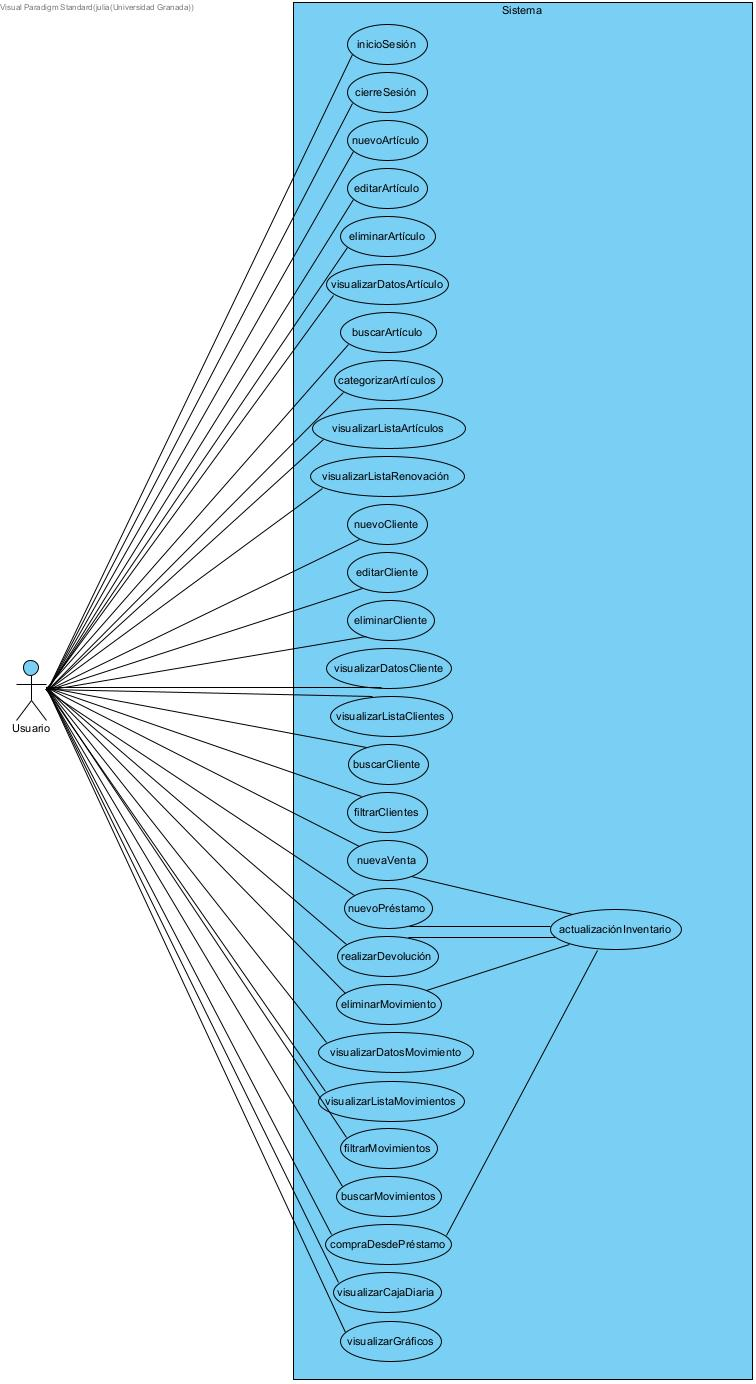
\includegraphics[width=0.88\textwidth]{imagenes/imagenesDiagramas/useCases.jpg}
	\caption{Diagrama de casos de uso}
	\label{fig:usecase}
\end{figure}

\newpage

\section{Modelos de comportamiento}

En esta sección vamos a especificar cómo opera el sistema ante las acciones del usuario mediante diagramas de secuencia. 

\subsection{Apertura y cierra de sesión}

\subsubsection{Inicio de sesión}

\begin{figure}[H]
	\centering
	\includegraphics[width=1\textwidth]{imagenes/imagenesDiagramas/InicioCierre/inicioSesión.jpg}
	\caption{Diagrama de secuencia de inicio de sesión}
	\label{fig:seqdiag1}
\end{figure}

\subsubsection{Cierre de sesión}

\begin{figure}[H]
	\centering
	\includegraphics[width=1\textwidth]{imagenes/imagenesDiagramas/InicioCierre/cierreSesión.jpg}
	\caption{Diagrama de secuencia de cierre de sesión}
	\label{fig:seqdiag2}
\end{figure}

\subsection{Gestión de artículos}

\subsubsection{Introducción de un nuevo artículo}

\begin{figure}[H]
	\centering
	\includegraphics[width=1\textwidth]{imagenes/imagenesDiagramas/Articulos/nuevoArtículo.jpg}
	\caption{Diagrama de secuencia de un nuevo artículo}
	\label{fig:seqdiag3}
\end{figure}

\subsubsection{Edición de un artículo existente}

\begin{figure}[H]
	\centering
	\includegraphics[width=1\textwidth]{imagenes/imagenesDiagramas/Articulos/editarArtículo.jpg}
	\caption{Diagrama de secuencia de edición de un artículo}
	\label{fig:seqdiag4}
\end{figure}

\subsubsection{Eliminación de un artículo}

\begin{figure}[H]
	\centering
	\includegraphics[width=1\textwidth]{imagenes/imagenesDiagramas/Articulos/eliminarArtículo.jpg}
	\caption{Diagrama de secuencia de eliminación de un artículo}
	\label{fig:seqdiag5}
\end{figure}

\subsubsection{Visualización de los datos de un artículo}

\begin{figure}[H]
	\centering
	\includegraphics[width=1\textwidth]{imagenes/imagenesDiagramas/Articulos/visualizarDatosArtículo.jpg}
	\caption{Diagrama de secuencia de visualización de datos de un artículo}
	\label{fig:seqdiag6}
\end{figure}

\subsubsection{Búsqueda de un artículo por nombre}

\begin{figure}[H]
	\centering
	\includegraphics[width=1\textwidth]{imagenes/imagenesDiagramas/Articulos/buscarArtículo.jpg}
	\caption{Diagrama de secuencia de búsqueda de un artículo}
	\label{fig:seqdiag7}
\end{figure}

\subsubsection{Categorización de un artículo}

\begin{figure}[H]
	\centering
	\includegraphics[width=1\textwidth]{imagenes/imagenesDiagramas/Articulos/categorizarArtículos.jpg}
	\caption{Diagrama de secuencia de categorización de un artículo}
	\label{fig:seqdiag8}
\end{figure}

\subsubsection{Visualización de la lista de artículos}

\begin{figure}[H]
	\centering
	\includegraphics[width=1\textwidth]{imagenes/imagenesDiagramas/Articulos/visualizarListaArtículos.jpg}
	\caption{Diagrama de secuencia de visualización de la lista de artículos}
	\label{fig:seqdiag9}
\end{figure}

\subsection{Gestión de inventario}

\subsubsection{Actualización del inventario de forma automática}

\begin{figure}[H]
	\centering
	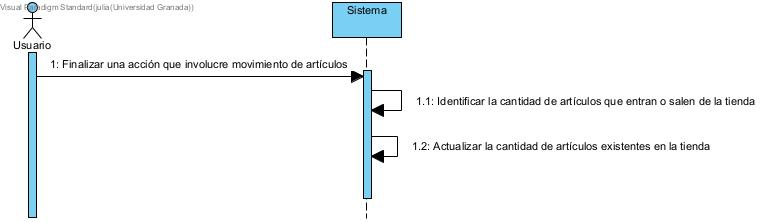
\includegraphics[width=1\textwidth]{imagenes/imagenesDiagramas/Articulos/actualizarInventario.jpg}
	\caption{Diagrama de secuencia de actualización de inventario}
	\label{fig:seqdiag10}
\end{figure}

\subsubsection{Visualización de la lista de renovación de artículos}

\begin{figure}[H]
	\centering
	\includegraphics[width=1\textwidth]{imagenes/imagenesDiagramas/Articulos/visualizarListaRenovación.jpg}
	\caption{Diagrama de secuencia de visualización de la lista de renovación de artículos}
	\label{fig:seqdiag11}
\end{figure}

\subsection{Gestión de clientes}

\subsubsection{Registro de un nuevo cliente habitual}

\begin{figure}[H]
	\centering
	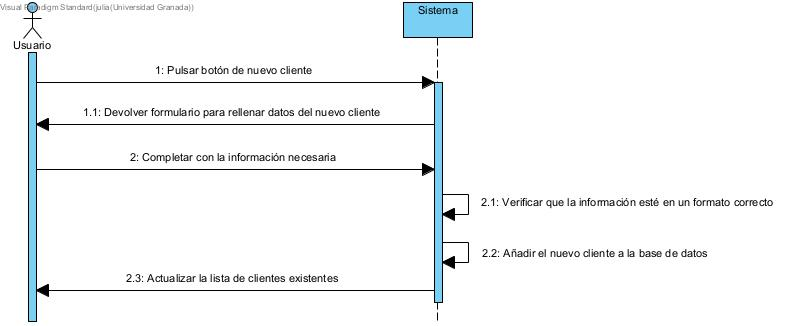
\includegraphics[width=1\textwidth]{imagenes/imagenesDiagramas/Cliente/nuevoCliente.jpg}
	\caption{Diagrama de secuencia de registro de un cliente}
	\label{fig:seqdiag12}
\end{figure}

\subsubsection{Edición de los datos de un cliente existente}

\begin{figure}[H]
	\centering
	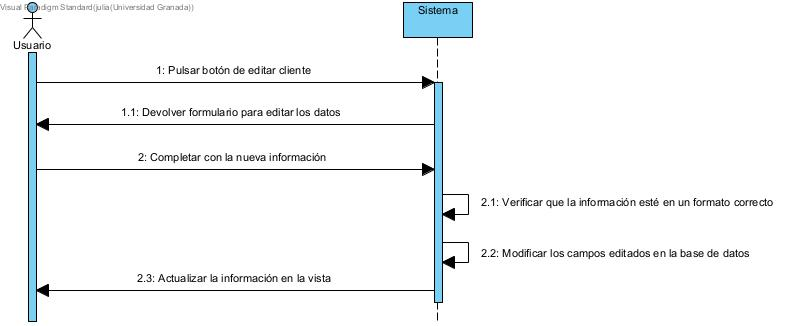
\includegraphics[width=1\textwidth]{imagenes/imagenesDiagramas/Cliente/editarCliente.jpg}
	\caption{Diagrama de secuencia de edición de los datos de un cliente}
	\label{fig:seqdiag13}
\end{figure}

\subsubsection{Eliminación de un cliente existente}

\begin{figure}[H]
	\centering
	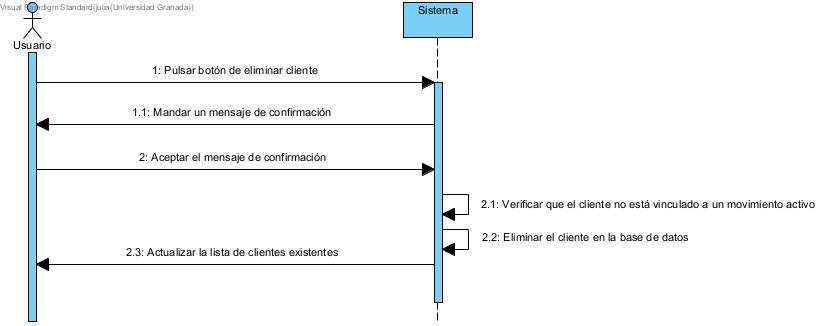
\includegraphics[width=1\textwidth]{imagenes/imagenesDiagramas/Cliente/eliminarCliente.jpg}
	\caption{Diagrama de secuencia de eliminación de un cliente}
	\label{fig:seqdiag14}
\end{figure}

\subsubsection{Visualización de los datos de un cliente}

\begin{figure}[H]
	\centering
	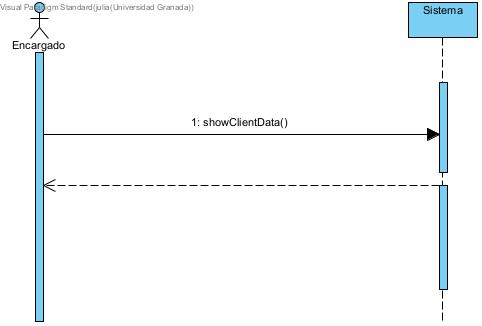
\includegraphics[width=1\textwidth]{imagenes/imagenesDiagramas/Cliente/visualizarDatosCliente.jpg}
	\caption{Diagrama de secuencia de visualización de los datos de un cliente}
	\label{fig:seqdiag15}
\end{figure}

\subsubsection{Visualización la lista de clientes existentes}

\begin{figure}[H]
	\centering
	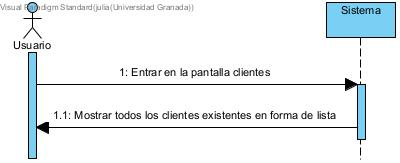
\includegraphics[width=1\textwidth]{imagenes/imagenesDiagramas/Cliente/visualizarListaClientes.jpg}
	\caption{Diagrama de secuencia de visualización de la lista de clientes}
	\label{fig:seqdiag16}
\end{figure}

\subsubsection{Búsqueda de un cliente por nombre}

\begin{figure}[H]
	\centering
	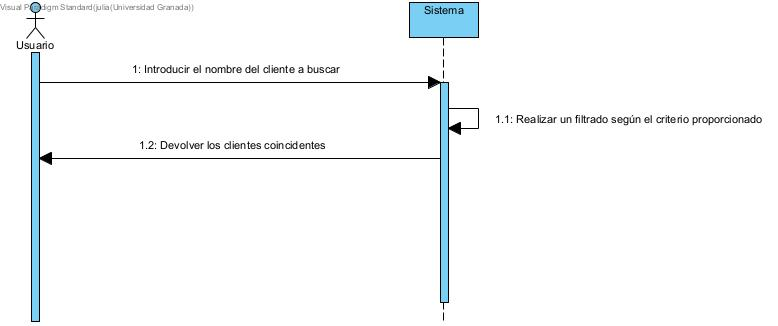
\includegraphics[width=1\textwidth]{imagenes/imagenesDiagramas/Cliente/buscarClientes.jpg}
	\caption{Diagrama de secuencia de búsqueda de un cliente}
	\label{fig:seqdiag17}
\end{figure}

\subsubsection{Filtrado de clientes con préstamos}

\begin{figure}[H]
	\centering
	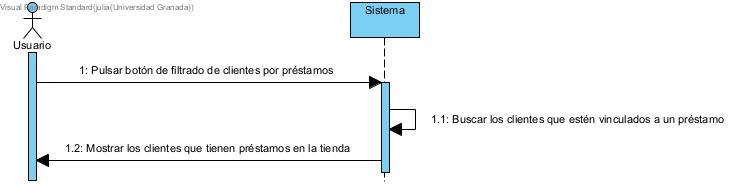
\includegraphics[width=1\textwidth]{imagenes/imagenesDiagramas/Cliente/filtrarClientes.jpg}
	\caption{Diagrama de secuencia de filtrado de clientes}
	\label{fig:seqdiag18}
\end{figure}

\subsection{Gestión de movimientos}

\subsubsection{Introducción de una nueva venta}

\begin{figure}[H]
	\centering
	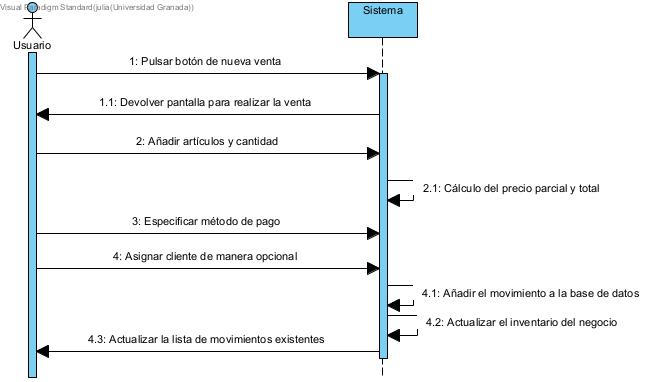
\includegraphics[width=1\textwidth]{imagenes/imagenesDiagramas/Movimientos/nuevaVenta.jpg}
	\caption{Diagrama de secuencia de nueva venta}
	\label{fig:seqdiag19}
\end{figure}

\subsubsection{Introducción de un nuevo préstamo}

\begin{figure}[H]
	\centering
	\includegraphics[width=1\textwidth]{imagenes/imagenesDiagramas/Movimientos/nuevoPréstamo.jpg}
	\caption{Diagrama de secuencia de nuevo préstamo}
	\label{fig:seqdiag20}
\end{figure}

\subsubsection{Introducción de una nueva devolución}

\begin{figure}[H]
	\centering
	\includegraphics[width=1\textwidth]{imagenes/imagenesDiagramas/Movimientos/realizarDevolución.jpg}
	\caption{Diagrama de secuencia de nueva devolución}
	\label{fig:seqdiag21}
\end{figure}

\subsubsection{Eliminación de un movimiento}

\begin{figure}[H]
	\centering
	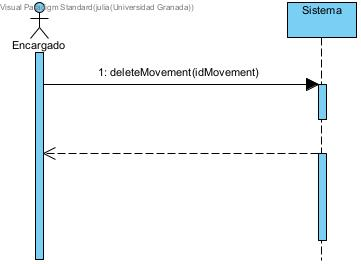
\includegraphics[width=1\textwidth]{imagenes/imagenesDiagramas/Movimientos/eliminarMovimiento.jpg}
	\caption{Diagrama de secuencia de eliminación de un movimiento}
	\label{fig:seqdiag22}
\end{figure}

\subsubsection{Visualización de los datos de un movimiento}

\begin{figure}[H]
	\centering
	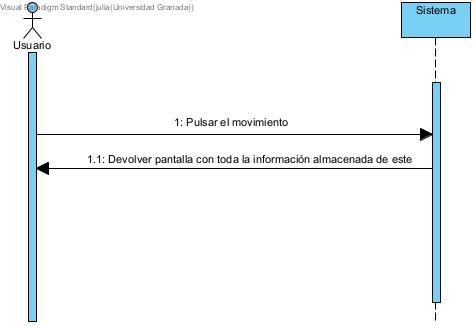
\includegraphics[width=1\textwidth]{imagenes/imagenesDiagramas/Movimientos/visualizarDatosMovimiento.jpg}
	\caption{Diagrama de secuencia de visualización de datos de un movimiento}
	\label{fig:seqdiag23}
\end{figure}

\subsubsection{Visualización de la lista de movimientos existentes}

\begin{figure}[H]
	\centering
	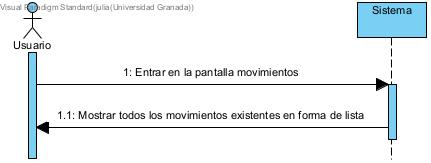
\includegraphics[width=1\textwidth]{imagenes/imagenesDiagramas/Movimientos/visualizarListaMovimientos.jpg}
	\caption{Diagrama de secuencia de visualización la lista de movimientos}
	\label{fig:seqdiag24}
\end{figure}

\subsubsection{Filtrado de los movimientos según su tipo}

\begin{figure}[H]
	\centering
	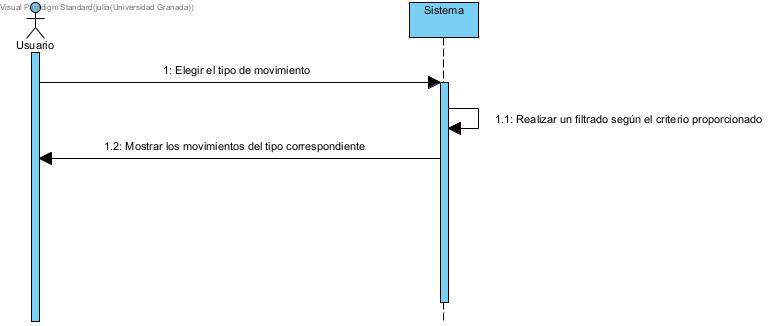
\includegraphics[width=1\textwidth]{imagenes/imagenesDiagramas/Movimientos/filtrarMovimientos.jpg}
	\caption{Diagrama de secuencia del filtrado de movimientos}
	\label{fig:seqdiag25}
\end{figure}

\subsubsection{Búsqueda de movimientos por fecha o cliente}

\begin{figure}[H]
	\centering
	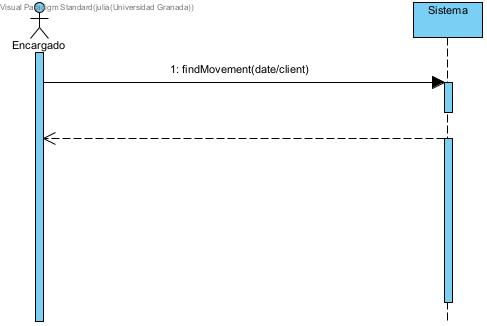
\includegraphics[width=1\textwidth]{imagenes/imagenesDiagramas/Movimientos/buscarMovimientos.jpg}
	\caption{Diagrama de secuencia de búsqueda de movimientos}
	\label{fig:seqdiag26}
\end{figure}

\subsubsection{Generación de una compra a partir de un préstamo}

\begin{figure}[H]
	\centering
	\includegraphics[width=1\textwidth]{imagenes/imagenesDiagramas/Movimientos/compraDesdePréstamo.jpg}
	\caption{Diagrama de secuencia de generación de una compra desde un préstamo}
	\label{fig:seqdiag27}
\end{figure}

\subsection{Gestión de resúmenes y gráficas}

\subsubsection{Visualización de la caja diaria}

\begin{figure}[H]
	\centering
	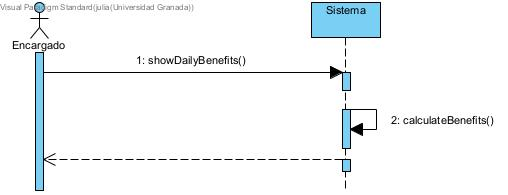
\includegraphics[width=1\textwidth]{imagenes/imagenesDiagramas/Graficos/visualizarCajaDiaria.jpg}
	\caption{Diagrama de secuencia de visualización de la caja diaria}
	\label{fig:seqdiag28}
\end{figure}

\subsubsection{Visualización de gráficos}

\begin{figure}[H]
	\centering
	\includegraphics[width=1\textwidth]{imagenes/imagenesDiagramas/Graficos/visualizarGráficos.jpg}
	\caption{Diagrama de secuencia de visualización de gráficos}
	\label{fig:seqdiag29}
\end{figure}


	
	\chapter{Diseño}
\label{chap:design}

\section{Diagrama de la arquitectura del sistema}

Como se puede observar en la imagen, la arquitectura del sistema es una arquitectura sencilla. El usuario interacciona únicamente con la interfaz gráfica de la aplicación y la aplicación solicita a la base de datos la información que el usuario requiere. De la misma forma, la base de datos envía la información a la aplicación y la aplicación se la muestra al usuario. El usuario y la base de datos no se relacionan directamente, siempre estará la aplicación como intermediario. 

No es necesaria la existencia de un servidor gracias a la herramienta que se está utilizando como base de datos, Supabase. Esta herramienta da servicio para construir aplicaciones software. 

\begin{figure}[ht]
	\centering
	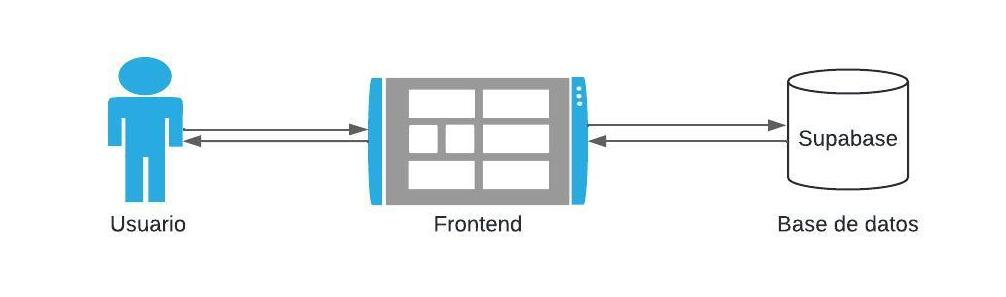
\includegraphics[width=1\textwidth]{imagenes/imagenesDiagramas/DiagramaArquitecturaSistema.jpeg}
	\caption{Diagrama de la arquitectura del sistema.}
	\label{fig:diagArquitectura}
\end{figure}

\newpage

\section{Diseño de la interfaz gráfica}

Debemos buscar la usabilidad y accesibilidad en una aplicación de estas características ya que el usuario final puede no tener grandes destrezas tecnológicas. Por tanto, hay que conseguir un diseño sencillo, fácil de usar e intuitivo. \\

Para ello, habrá que tener en cuenta los siguientes criterios:

\begin{itemize}
	\item \textbf{Botones grandes:} Los botones de la aplicación deben de tener un tamaño adecuado para facilitar la realización de acciones. 
	\item \textbf{Tamaño y contraste del texto:} Nos debemos de asegurar que el tamaño de la letra es lo suficientemente grande y que el contraste con el fondo es significativo para facilitar con ello la lectura. El fondo de la aplicación será blanco para conseguir un buen contraste y evitar las distracciones. 
	\item \textbf{Claridad en la navegación:} Proporcionar una estructura lógica de navegación y unas flechas visibles que permitan cambiar de pantallas de manera intuitiva. 
	\item \textbf{Simplicidad:} El diseño debe ser sencillo. Evitar la sobrecarga de información y priorizar un diseño ordenado. 
	\item \textbf{Feedback:} La aplicación debe proporcionar una respuesta a las acciones del usuario para confirmar que se realizan de manera correcta. 
\end{itemize} 

\newpage

\subsection{Pantalla de inicio de sesión}

En esta sección se muestra el boceto de la interfaz gráfica del inicio de sesión. Se corresponde con el requisito RF1. 

\begin{figure}[ht]
	\centering
	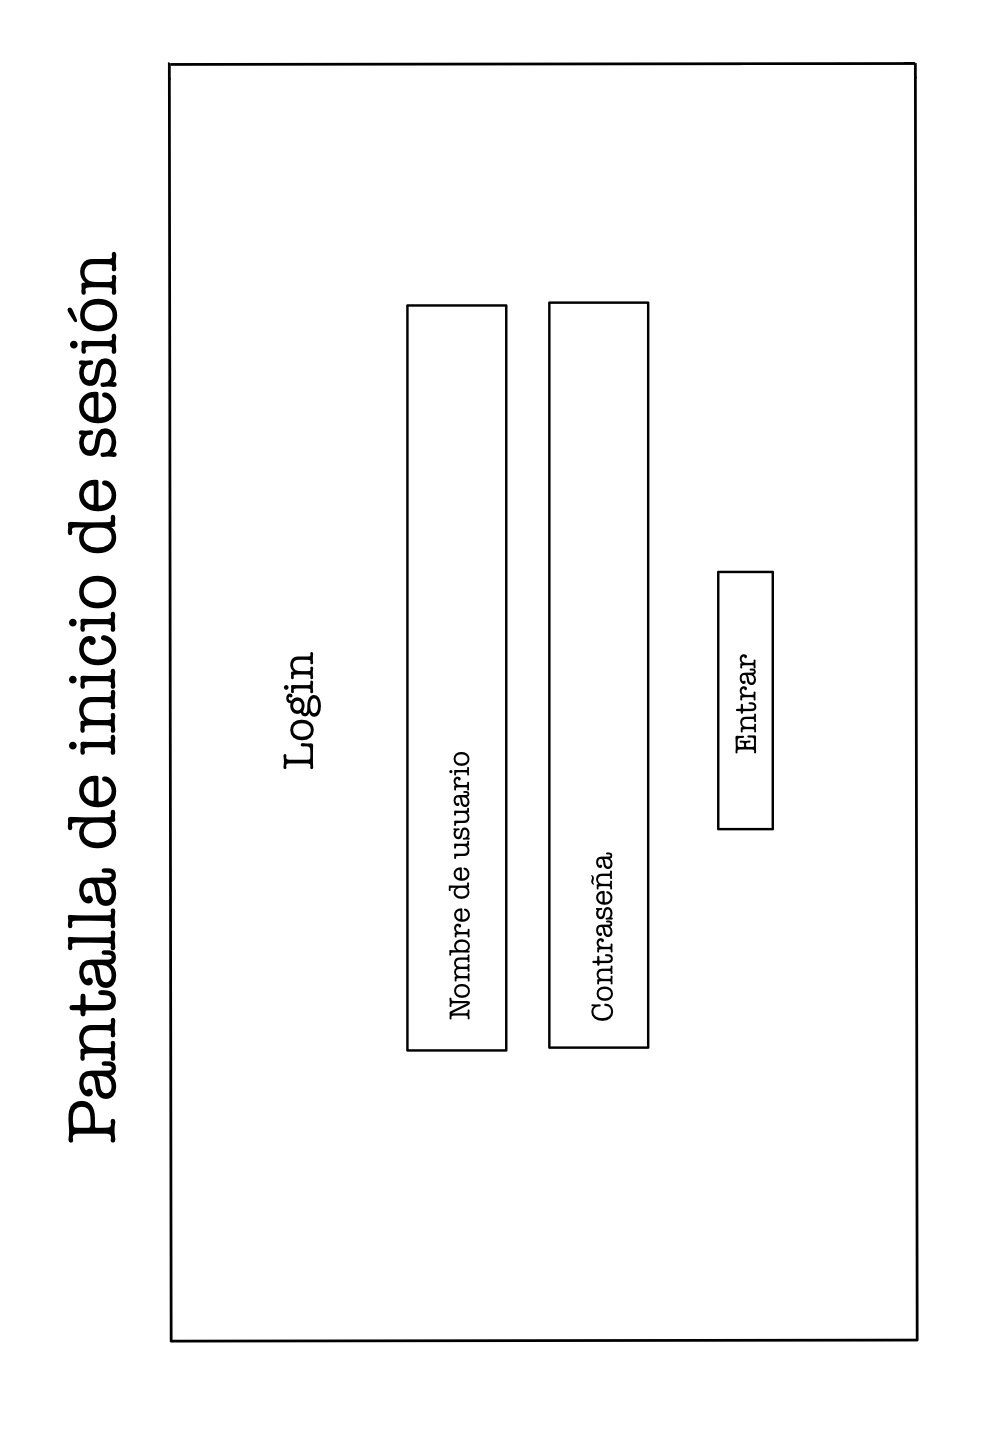
\includegraphics[width=0.7\textwidth, angle=270]{imagenes/inicio_sesion.JPG}
	\caption{Diseño de la pantalla de inicio de sesión.}
	\label{fig:iniciosesion}
\end{figure}

\newpage

\subsection{Pantalla principal}

En esta sección se muestran los bocetos de la interfaz gráfica de la pantalla principal y las pantallas correspondientes con una nueva venta y un nuevo préstamo. Estas tres pantallas representan los requisitos RF19, RF20 y RF28. Por tanto, es la pantalla que muestra la caja diaria y permite registrar una nueva venta o un nuevo préstamo. 

\begin{figure}[ht]
	\centering
	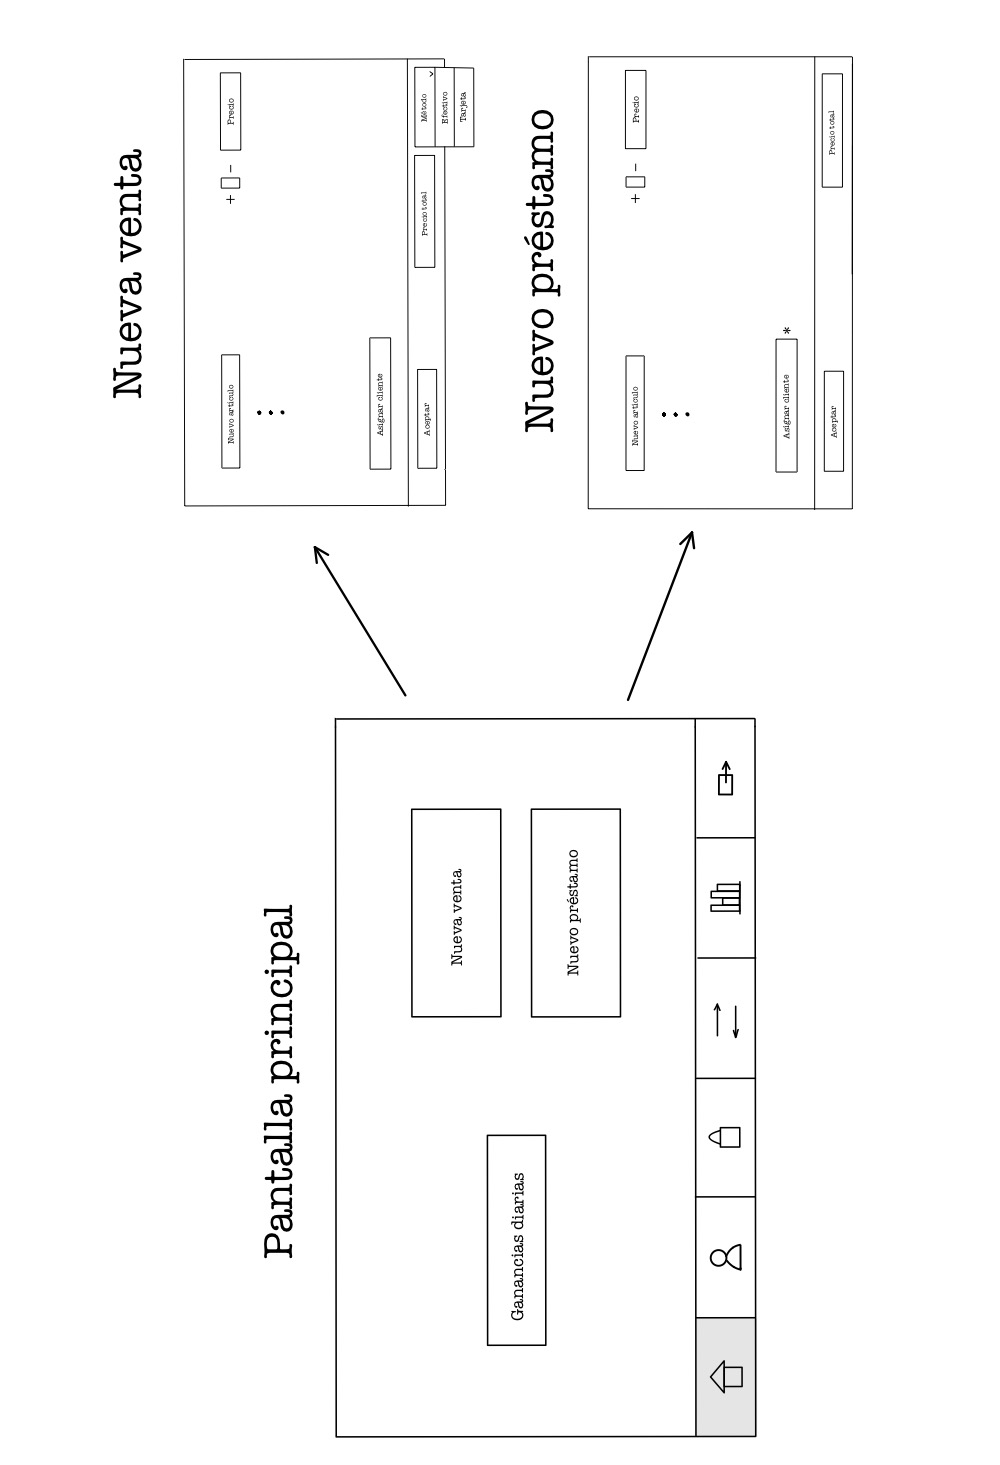
\includegraphics[width=0.8\textwidth, angle=270]{imagenes/pantalla_principal.JPG}
	\caption{Diseño de la pantalla principal.}
	\label{fig:pantallaprincipal}
\end{figure}

\newpage

\subsection{Pantalla de clientes}

En esta sección se muestran los bocetos de la interfaz gráfica de la pantalla clientes. Estas cuatro pantallas representan los requisitos RF12, RF13, RF14, RF15, RF16, RF17 y RF18. En la pantalla clientes podemos ver la lista de clientes existentes, buscar clientes por nombre y filtrar aquellos clientes que tengan préstamos. Si pulsamos encima del nombre del cliente, visualizaremos todos los datos relacionados con este. Además, podemos editar, eliminar y añadir un nuevo cliente. 


\begin{figure}[ht]
	\centering
	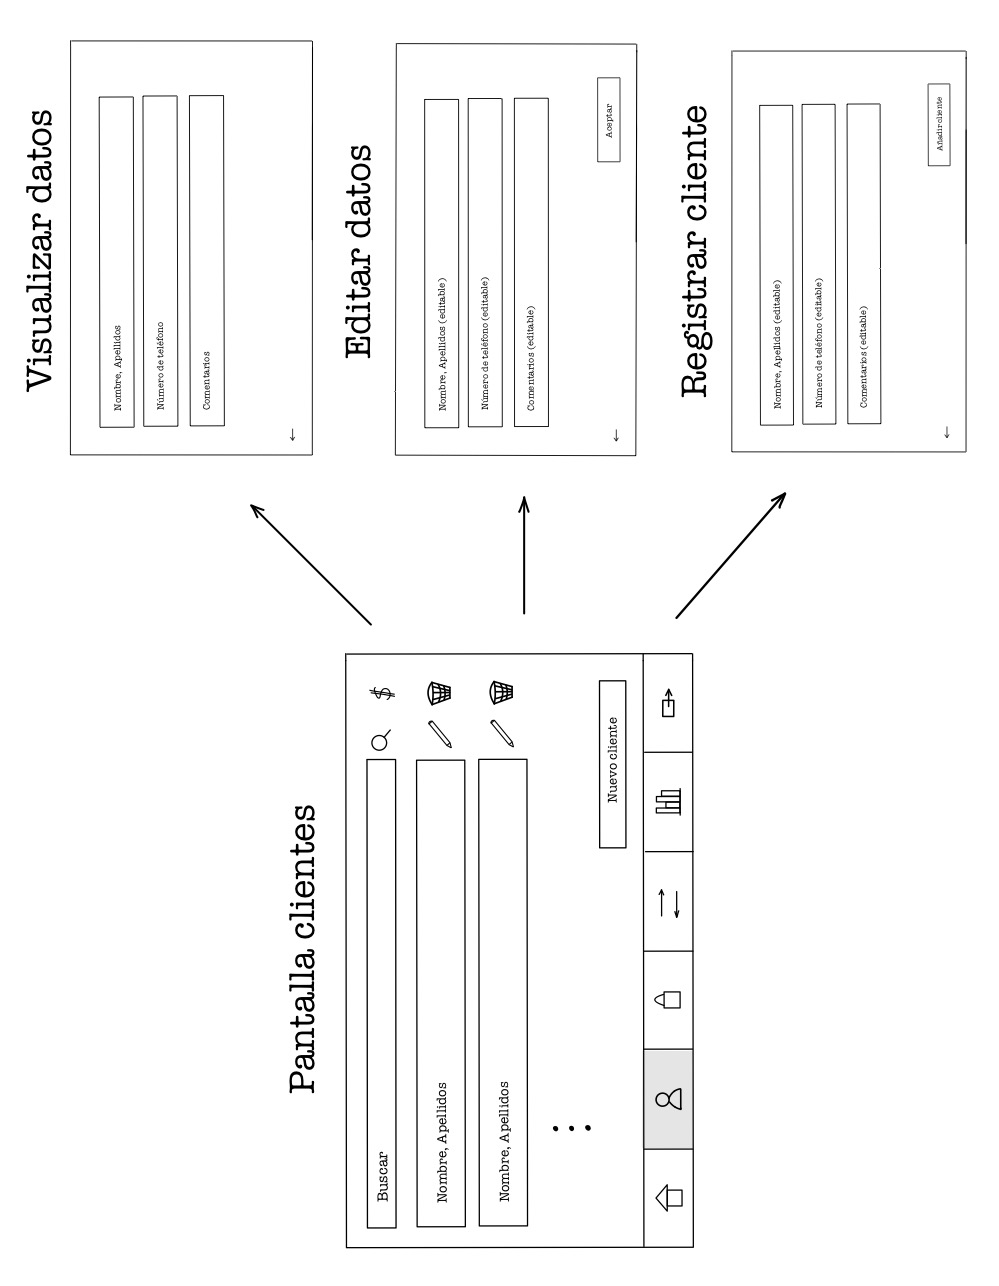
\includegraphics[width=0.8\textwidth, angle=270]{imagenes/pantalla_clientes.JPG}
	\caption{Diseño de la pantalla clientes.}
	\label{fig:pantallaclientes}
\end{figure}

\newpage

\subsection{Pantalla de artículos}

En esta sección se muestran los bocetos de la interfaz gráfica de la pantalla artículos. Estas cinco pantallas representan los requisitos RF3, RF4, RF5, RF6, RF7, RF8, RF9, RF10 y RF11. En la pantalla artículos podemos ver la lista de artículos existentes, buscar los artículos por nombre y filtrarlos por categoría. Si pulsamos encima del nombre del artículo, visualizaremos todos los datos relacionados con este. Además, podemos editar, eliminar y añadir un nuevo artículo. Por último, tenemos la lista de renovación de stock donde se introducirán todos los artículos que deba comprar el comerciante. 


\begin{figure}[ht]
	\centering
	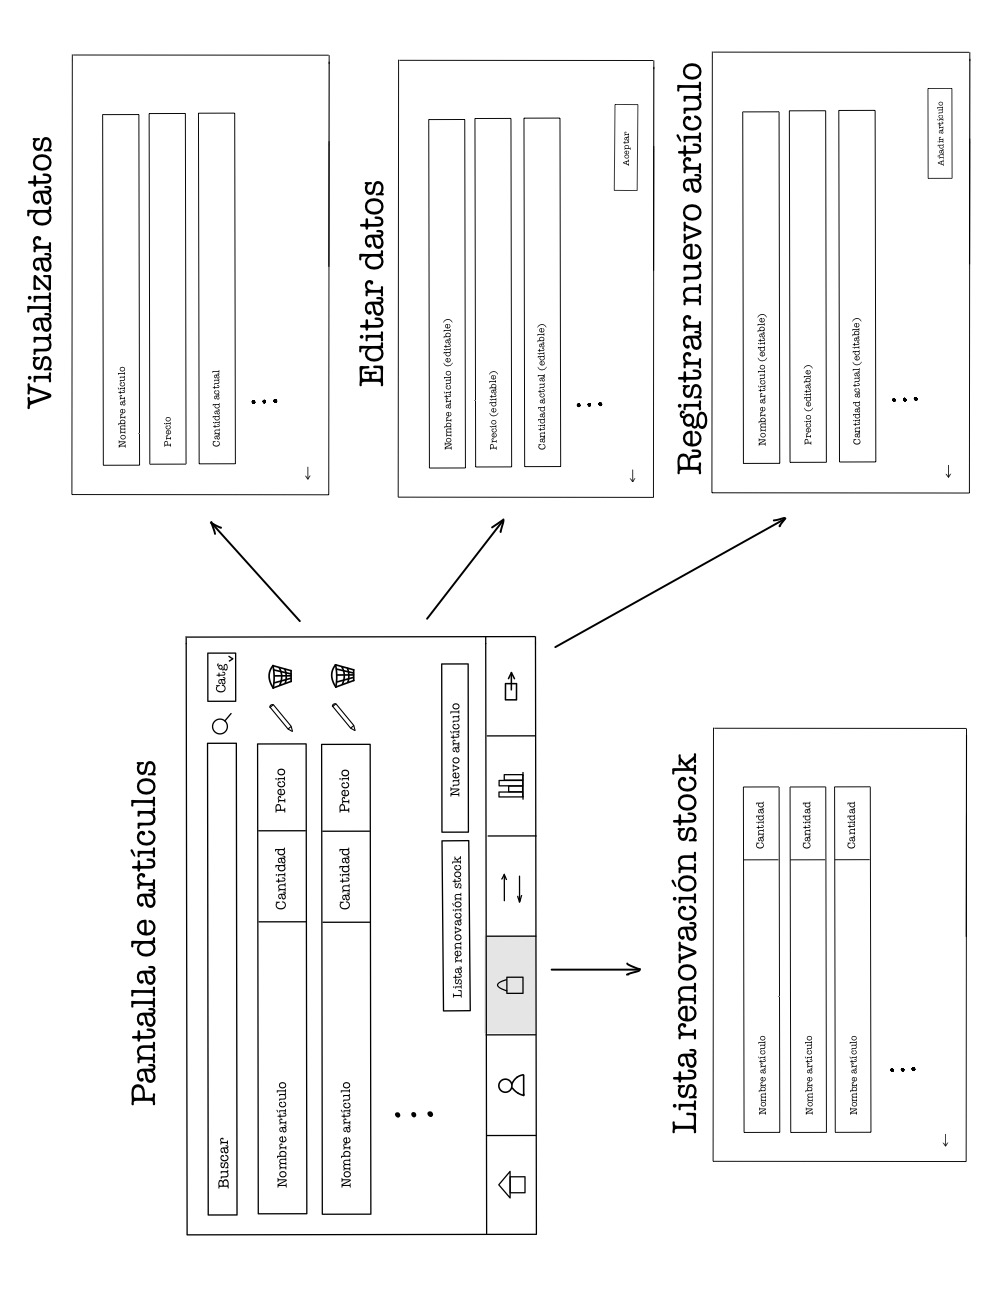
\includegraphics[width=0.8\textwidth, angle=270]{imagenes/pantalla_articulos.JPG}
	\caption{Diseño de la pantalla artículos.}
	\label{fig:pantallaarticulos}
\end{figure}

\newpage


\subsection{Pantalla de movimientos}

En esta sección se muestran los bocetos de la interfaz gráfica de la pantalla movimientos. Estas cuatro pantallas representan los requisitos RF21, RF22, RF23, RF24, RF25, RF26 y RF27. En la pantalla movimientos podemos ver la lista de movimientos existentes, buscar los movimientos por fecha o cliente asignado y filtrarlos por tipo de movimiento (venta, préstamo o devolución). Si pulsamos encima del movimiento, visualizaremos todos los datos relacionados con este. Si el movimiento es de tipo "préstamo", además de visualizarlo podremos convertirlo en venta seleccionando aquellos artículos que el cliente desea comprar. Únicamente se podrán devolver las ventas, ya que son los movimientos que generan una subida económica en la caja diaria. Las devoluciones generan una bajada correspondiente con la cantidad devuelta. Si se devuelve un préstamo sin comprar nada, se elimina el movimiento. Podemos eliminar cualquier movimiento, sea del tipo que sea. 


\begin{figure}[ht]
	\centering
	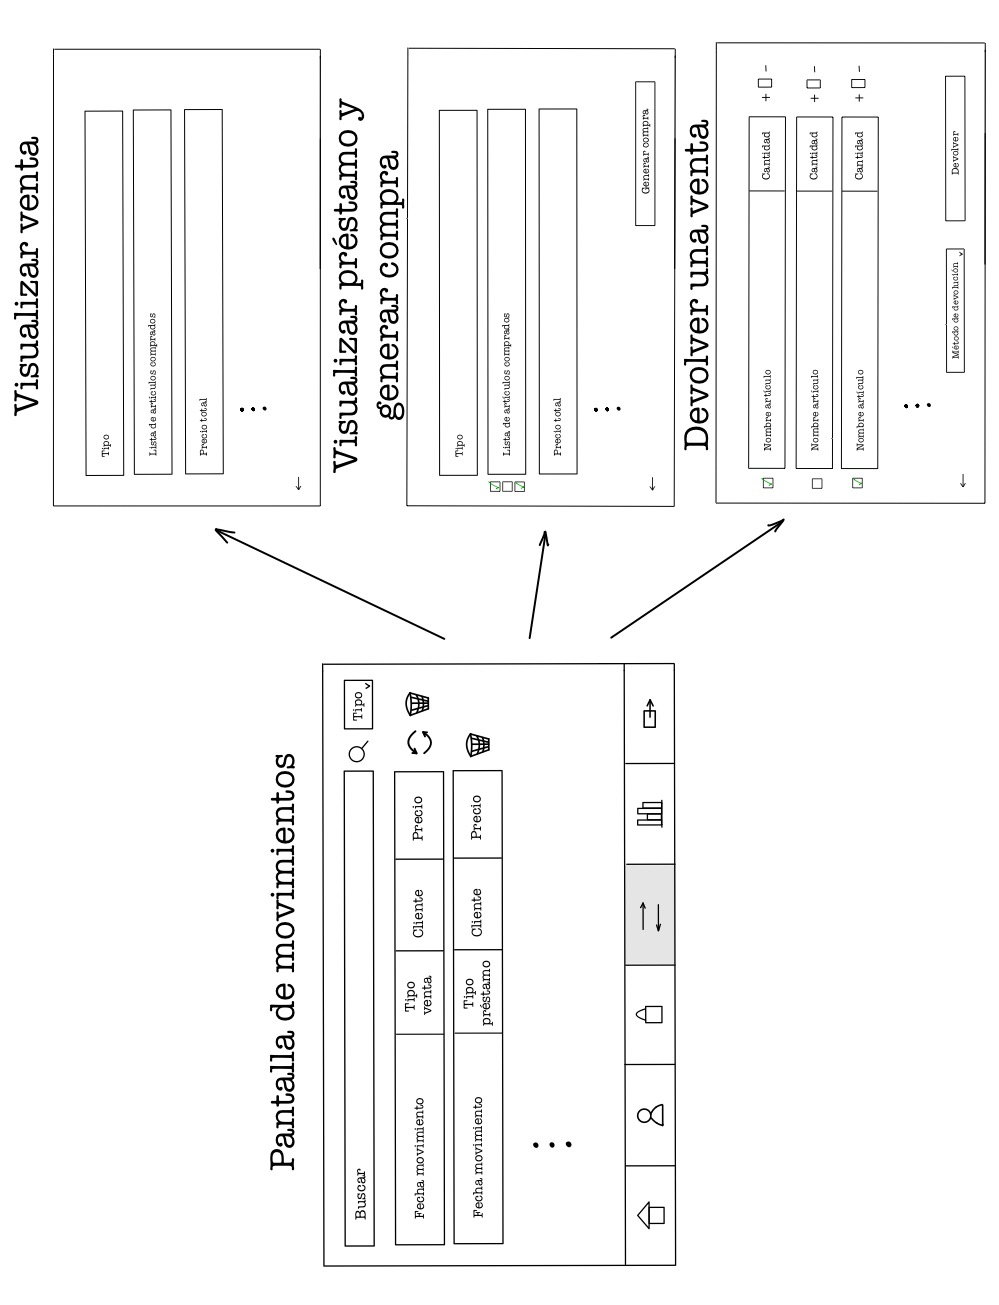
\includegraphics[width=0.8\textwidth, angle=270]{imagenes/pantalla_movimientos.JPG}
	\caption{Diseño de la pantalla movimientos.}
	\label{fig:pantallamovimientos}
\end{figure}

\newpage

\subsection{Pantalla de gráficos y cierre de sesión}

En esta sección se muestra el boceto de la interfaz gráfica de la pantalla gráficos. Esta pantalla representa el requisito RF29. Aquí podemos observar el progreso económico del negocio en forma de gráfica. Podremos verlo de forma mensual o anual. 

Para finalizar, el cierre de sesión podrá hacerse desde cualquier lugar simplemente pulsando en su botón. Esto corresponde con el requisito RF2. 


\begin{figure}[ht]
	\centering
	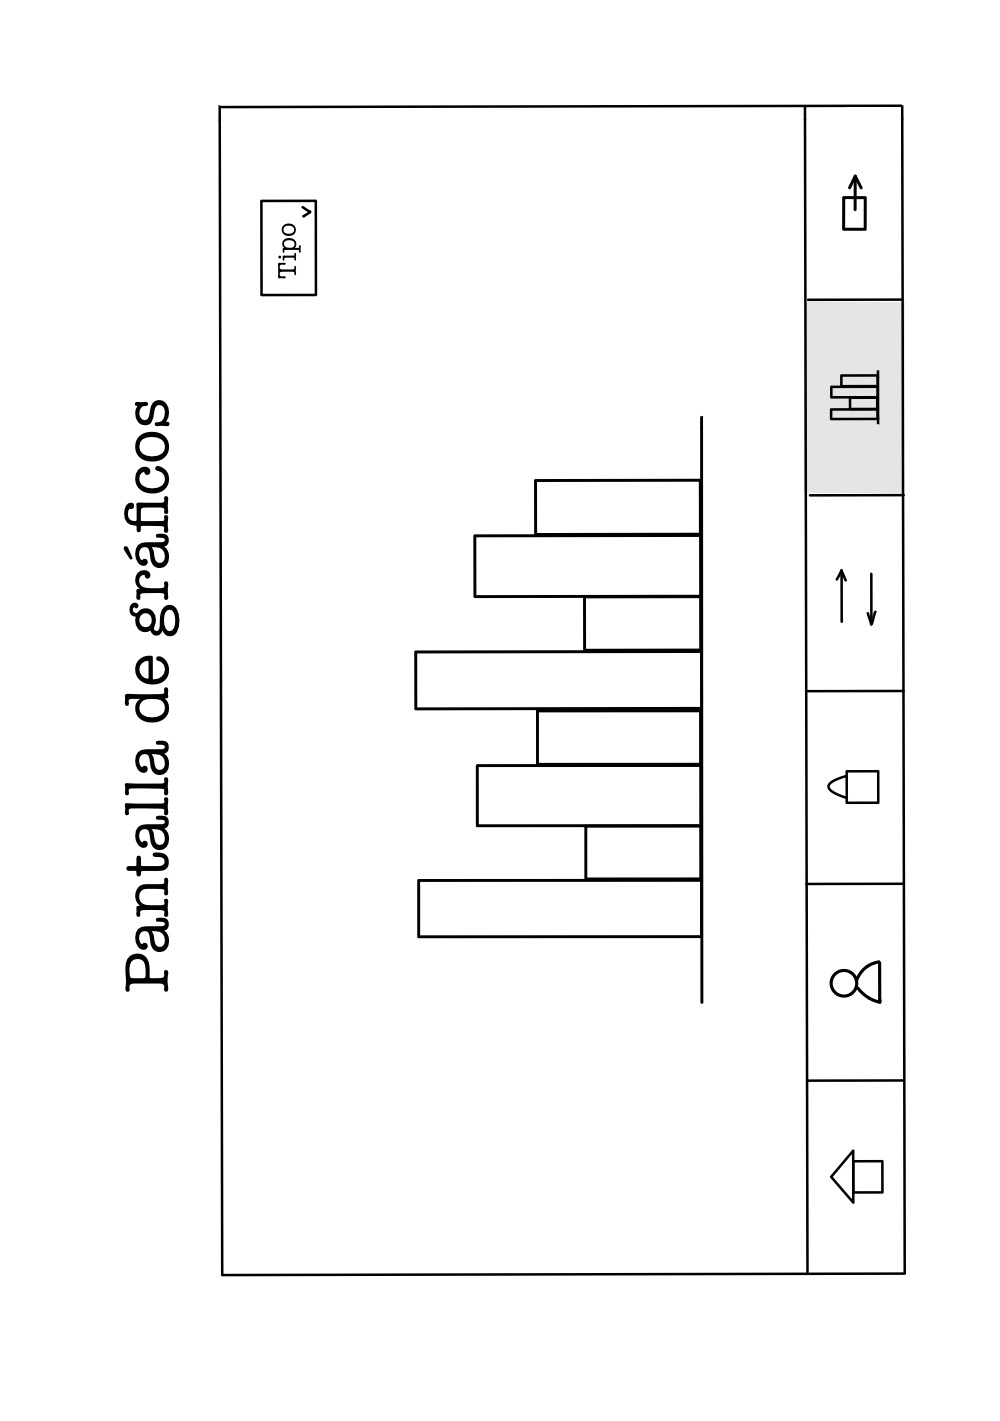
\includegraphics[width=0.8\textwidth, angle=270]{imagenes/pantalla_graficos.JPG}
	\caption{Diseño de la pantalla gráficos.}
	\label{fig:pantallagraficos}
\end{figure}
	
	\chapter{Anexo 1}
\label{chap:appvalidation}
	
	\newpage
	
	\bibliography{bibliografia}
	
\end{document}




%
%
%\input{capitulos/03_Requisitos}
%
%\chapter{Análisis}
\label{chap:analysis}

\section{Especificación de requisitos}

Dentro del desarrollo de un proyecto, la fase de especificación de requisitos cumple un rol fundamental, ya que será aquí donde se establezcan las características esenciales y las expectativas que debe cumplir el sistema. 

Esta sección está dedicada a la identificación y descripción detallada de los requisitos. Para conseguir este fin, es necesario preguntar al cliente y stakeholders sobre las necesidades o limitaciones que esperan del software.\\
 
Cada requisito se identificará de forma única mediante un código que indica el tipo de requisito y su número correspondiente. Mediante esta codificación podremos hacer referencia a los requisitos de forma sencilla a lo largo de este documento. 


\subsection{Requisitos funcionales}

Los requisitos funcionales son aquellos que definen las tareas específicas que el sistema debe ser capaz de realizar. Podemos ordenar estos requisitos en 6 grupos según la función que habilitan: 

\begin{itemize}
	\item \textbf{Grupo 1:} Apertura y cierre de sesión. 
	\item \textbf{Grupo 2:} Gestión de artículos.
	\item \textbf{Grupo 3:} Gestión de inventario. 
	\item \textbf{Grupo 4:} Gestión de clientes. 
	\item \textbf{Grupo 5:} Gestión de movimientos.
	\item \textbf{Grupo 6:} Gestión de resúmenes y gráficas. 
\end{itemize}

A continuación se especificarán los requisitos funcionales del proyecto clasificándolos en las secciones anteriormente mencionadas. 


\subsubsection{Apertura y cierra de sesión}

% Tabla para el inicio de sesión
\begin{table}[htb!]
	\centering % Centra la tabla en la página
	\begin{tabular}{|p{0.35\linewidth}|p{0.6\linewidth}|}
		\hline
		\rowcolor{grayshade} \textbf{RF1} & \textbf{Inicio de sesión} \\
		\hline
		\textbf{Prioridad} & Alta \\
		\hline
		\textbf{Descripción} & El sistema debe permitir al usuario iniciar sesión de forma segura.  \\
		\hline
		\vspace{0.5mm}
		\textbf{Criterios de aceptación} & 
		\begin{minipage}[t]{0.9\linewidth}
			\begin{enumerate}
				\item La pantalla de inicio de sesión debe pedir el nombre de usuario y la contraseña.
				\item Verificar que los campos no estén vacíos.
				\item Verificar que la información introducida es correcta y autentica al usuario.
				\item Si la información es incorrecta, mostrar un mensaje de error.
				\item Tras el inicio de sesión, redirigir al usuario a la pantalla principal.
			\end{enumerate}
			\vspace{2mm}
		\end{minipage} \\
		\hline
	\end{tabular}
	\caption{RF1}
\end{table}

\newpage

% Tabla para el cierre de sesión
\begin{table}[htb!]
	\centering % Centra la tabla en la página
	\begin{tabular}{|p{0.35\linewidth}|p{0.6\linewidth}|}
		\hline
		\rowcolor{grayshade} \textbf{RF2} & \textbf{Cierre de sesión} \\
		\hline
		\textbf{Prioridad} & Alta \\
		\hline
		\textbf{Descripción} & El sistema debe permitir al usuario cerrar sesión de forma segura.  \\
		\hline
		\vspace{0.5mm}
		\textbf{Criterios de aceptación} & 
		\begin{minipage}[t]{0.9\linewidth}
			\begin{enumerate}
				\item Debe existir una opción visible para cerrar la sesión.
				\item Tras el cierre de sesión, se debe volver a la pantalla de inicio de sesión.
			\end{enumerate}
			\vspace{2mm}
		\end{minipage} \\
		\hline
	\end{tabular}
	\caption{RF2}
\end{table}

\subsubsection{Gestión de artículos}

% Tabla para añadir un nuevo artículo.
\begin{table}[htb!]
	\centering % Centra la tabla en la página
	\begin{tabular}{|p{0.35\linewidth}|p{0.6\linewidth}|}
		\hline
		\rowcolor{grayshade} \textbf{RF3} & \textbf{Introducción de un nuevo artículo} \\
		\hline
		\textbf{Prioridad} & Alta \\
		\hline
		\textbf{Descripción} & El sistema debe permitir registrar un nuevo artículo al negocio.\\
		\hline
		\vspace{0.5mm}
		\textbf{Criterios de aceptación} & 
		\begin{minipage}[t]{0.9\linewidth}
			\begin{enumerate}
				\item Debe existir una opción visible para añadir un nuevo artículo.
				\item Verificar que los campos obligatorios no están vacíos.
				\item Verificar que la información introducida tenga un formato correcto.
				\item Tras guardar un nuevo artículo, se debe actualizar la lista de artículos existente. 
			\end{enumerate}
			\vspace{2mm}
		\end{minipage} \\
		\hline
	\end{tabular}
	\caption{RF3}
\end{table}

% Tabla para editar un nuevo artículo existente.
\begin{table}[htb!]
	\centering % Centra la tabla en la página
	\begin{tabular}{|p{0.35\linewidth}|p{0.6\linewidth}|}
		\hline
		\rowcolor{grayshade} \textbf{RF4} & \textbf{Edición de un artículo existente} \\
		\hline
		\textbf{Prioridad} & Alta \\
		\hline
		\textbf{Descripción} & El sistema debe permitir editar los datos de un artículo existente.\\
		\hline
		\vspace{0.5mm}
		\textbf{Criterios de aceptación} & 
		\begin{minipage}[t]{0.9\linewidth}
			\begin{enumerate}
				\item Debe existir una opción visible para editar un artículo existente.
				\item Verificar que la nueva información introducida tenga un formato correcto.
				\item Tras guardar los cambios, se deben actualizar los campos en la base de datos. 
			\end{enumerate}
			\vspace{2mm}
		\end{minipage} \\
		\hline
	\end{tabular}
	\caption{RF4}
\end{table}

% Tabla para eliminar un nuevo artículo existente.
\begin{table}[htb!]
	\centering % Centra la tabla en la página
	\begin{tabular}{|p{0.35\linewidth}|p{0.6\linewidth}|}
		\hline
		\rowcolor{grayshade} \textbf{RF5} & \textbf{Eliminación de un artículo} \\
		\hline
		\textbf{Prioridad} & Alta \\
		\hline
		\textbf{Descripción} & El sistema debe permitir eliminar un artículo existente.\\
		\hline
		\vspace{0.5mm}
		\textbf{Criterios de aceptación} & 
		\begin{minipage}[t]{0.9\linewidth}
			\begin{enumerate}
				\item Debe existir una opción visible para eliminar un artículo existente.
				\item Mandar un mensaje de confirmación antes de la eliminación. 
				\item Verificar que el artículo no esté vinculado a movimientos existentes en la base de datos.
				\item Tras eliminar el artículo correspondiente, actualizar la lista de artículos existentes. 
			\end{enumerate}
			\vspace{2mm}
		\end{minipage} \\
		\hline
	\end{tabular}
	\caption{RF5}
\end{table}

% Tabla para buscar un artículo.
\begin{table}[htb!]
	\centering % Centra la tabla en la página
	\begin{tabular}{|p{0.35\linewidth}|p{0.6\linewidth}|}
		\hline
		\rowcolor{grayshade} \textbf{RF6} & \textbf{Búsqueda de un artículo por nombre} \\
		\hline
		\textbf{Prioridad} & Alta \\
		\hline
		\textbf{Descripción} & El sistema debe permitir buscar un artículo por nombre.\\
		\hline
		\vspace{0.5mm}
		\textbf{Criterios de aceptación} & 
		\begin{minipage}[t]{0.9\linewidth}
			\begin{enumerate}
				\item Debe existir una opción visible para buscar un artículo existente.
				\item El usuario debe introducir el nombre correcto que identifica el artículo. 
				\item El sistema debe mostrar al usuario el/los artículos que están relacionados con la búsqueda. 
			\end{enumerate}
			\vspace{2mm}
		\end{minipage} \\
		\hline
	\end{tabular}
	\caption{RF6}
\end{table}

% Tabla para categorizar un artículo.
\begin{table}[htb!]
	\centering % Centra la tabla en la página
	\begin{tabular}{|p{0.35\linewidth}|p{0.6\linewidth}|}
		\hline
		\rowcolor{grayshade} \textbf{RF7} & \textbf{Categorización de un artículo} \\
		\hline
		\textbf{Prioridad} & Alta \\
		\hline
		\textbf{Descripción} & El sistema debe ser capaz de ordenar los artículos en categorías.\\
		\hline
		\vspace{0.5mm}
		\textbf{Criterios de aceptación} & 
		\begin{minipage}[t]{0.9\linewidth}
			\begin{enumerate}
				\item El usuario debe establecer la categoría del artículo de forma correcta.
				\item El sistema debe ordenar los artículos en base a las categorías especificadas. 
			\end{enumerate}
			\vspace{2mm}
		\end{minipage} \\
		\hline
	\end{tabular}
	\caption{RF7}
\end{table}

% Tabla para mostrar la lista de artículos existentes.
\begin{table}[htb!]
	\centering % Centra la tabla en la página
	\begin{tabular}{|p{0.35\linewidth}|p{0.6\linewidth}|}
		\hline
		\rowcolor{grayshade} \textbf{RF8} & \textbf{Visualización de la lista de artículos existentes} \\
		\hline
		\textbf{Prioridad} & Alta \\
		\hline
		\textbf{Descripción} & El sistema debe ser capaz de mostrar una lista con los artículos del negocio.\\
		\hline
		\vspace{0.5mm}
		\textbf{Criterios de aceptación} & 
		\begin{minipage}[t]{0.9\linewidth}
			\begin{enumerate}
				\item El sistema debe ser capaz de mostrar los artículos existentes en la base de datos en una lista. 
			\end{enumerate}
			\vspace{2mm}
		\end{minipage} \\
		\hline
	\end{tabular}
	\caption{RF8}
\end{table}

\clearpage

\subsubsection{Gestión de inventario}

% Tabla para actualizar el inventario de forma automática.
\begin{table}[H]
	\centering % Centra la tabla en la página
	\begin{tabular}{|p{0.35\linewidth}|p{0.6\linewidth}|}
		\hline
		\rowcolor{grayshade} \textbf{RF9} & \textbf{Actualización del inventario de forma automática} \\
		\hline
		\textbf{Prioridad} & Alta \\
		\hline
		\textbf{Descripción} & El sistema debe ser capaz de actualizar el inventario de los artículos del negocio en tiempo real.\\
		\hline
		\vspace{0.5mm}
		\textbf{Criterios de aceptación} & 
		\begin{minipage}[t]{0.9\linewidth}
			\begin{enumerate}
				\item El sistema debe ser capaz de actualizar las cantidades de los artículos existentes en base a los movimientos (ventas, devoluciones o préstamos) del negocio. 
			\end{enumerate}
			\vspace{2mm}
		\end{minipage} \\
		\hline
	\end{tabular}
	\caption{RF9}
\end{table}

% Tabla para visualización de la lista de renovación de artículos.
\begin{table}[H]
	\centering % Centra la tabla en la página
	\begin{tabular}{|p{0.35\linewidth}|p{0.6\linewidth}|}
		\hline
		\rowcolor{grayshade} \textbf{RF10} & \textbf{Visualización de lista de renovación de artículos} \\
		\hline
		\textbf{Prioridad} & Media \\
		\hline
		\textbf{Descripción} & El sistema debe ser capaz de realizar una lista con los artículos que lleguen a una cantidad crítica para indicar al comerciante que debe comprar más stock.\\
		\hline
		\vspace{0.5mm}
		\textbf{Criterios de aceptación} & 
		\begin{minipage}[t]{0.9\linewidth}
			\begin{enumerate}
				\item Debe existir una opción visible para visualizar la lista.
				\item El sistema debe introducir el artículo en la lista cada vez que la cantidad actual sea igual o inferior a la cantidad mínima establecida por el comerciante. 
			\end{enumerate}
			\vspace{2mm}
		\end{minipage} \\
		\hline
	\end{tabular}
	\caption{RF10}
\end{table}

\subsubsection{Gestión de clientes}

% Tabla para registrar un nuevo cliente.
\begin{table}[H]
	\centering % Centra la tabla en la página
	\begin{tabular}{|p{0.35\linewidth}|p{0.6\linewidth}|}
		\hline
		\rowcolor{grayshade} \textbf{RF11} & \textbf{Registro de un nuevo cliente habitual} \\
		\hline
		\textbf{Prioridad} & Alta \\
		\hline
		\textbf{Descripción} & El sistema debe permitir añadir un nuevo cliente al sistema.\\
		\hline
		\vspace{0.5mm}
		\textbf{Criterios de aceptación} & 
		\begin{minipage}[t]{0.9\linewidth}
			\begin{enumerate}
				\item Debe existir una opción visible para añadir un nuevo cliente. 
				\item Verificar que los campos obligatorios no estén vacíos. 
				\item Verificar que la información proporcionada tenga un formato correcto. 
				\item Añadir el nuevo cliente a la base de datos y actualizar la lista de clientes existentes. 
			\end{enumerate}
			\vspace{2mm}
		\end{minipage} \\
		\hline
	\end{tabular}
	\caption{RF11}
\end{table}

% Tabla para editar los datos de un cliente.
\begin{table}[H]
	\centering % Centra la tabla en la página
	\begin{tabular}{|p{0.35\linewidth}|p{0.6\linewidth}|}
		\hline
		\rowcolor{grayshade} \textbf{RF12} & \textbf{Edición de los datos de un cliente existente} \\
		\hline
		\textbf{Prioridad} & Alta \\
		\hline
		\textbf{Descripción} & El sistema debe permitir editar los datos de un cliente existente.\\
		\hline
		\vspace{0.5mm}
		\textbf{Criterios de aceptación} & 
		\begin{minipage}[t]{0.9\linewidth}
			\begin{enumerate}
				\item Debe existir una opción visible para editar los datos de un cliente. 
				\item Verificar que la nueva información proporcionada tenga un formato correcto. 
				\item Tras confirmar los cambios, editar los campos modificados en la base de datos.
			\end{enumerate}
			\vspace{2mm}
		\end{minipage} \\
		\hline
	\end{tabular}
	\caption{RF12}
\end{table}

% Tabla para eliminar un cliente existente.
\begin{table}[H]
	\centering % Centra la tabla en la página
	\begin{tabular}{|p{0.35\linewidth}|p{0.6\linewidth}|}
		\hline
		\rowcolor{grayshade} \textbf{RF13} & \textbf{Eliminación de un cliente existente} \\
		\hline
		\textbf{Prioridad} & Alta \\
		\hline
		\textbf{Descripción} & El sistema debe permitir eliminar un cliente existente.\\
		\hline
		\vspace{0.5mm}
		\textbf{Criterios de aceptación} & 
		\begin{minipage}[t]{0.9\linewidth}
			\begin{enumerate}
				\item Debe existir una opción visible para eliminar un cliente. 
				\item Mandar un mensaje de confirmación antes de la eliminación. 
				\item Verificar que el cliente no esté vinculado a ningún movimiento activo.
				\item Tras eliminar al cliente, actualizar la lista de clientes existentes. 
			\end{enumerate}
			\vspace{2mm}
		\end{minipage} \\
		\hline
	\end{tabular}
	\caption{RF13}
\end{table}

% Tabla para visualizar la lista de clientes actuales.
\begin{table}[H]
	\centering % Centra la tabla en la página
	\begin{tabular}{|p{0.35\linewidth}|p{0.6\linewidth}|}
		\hline
		\rowcolor{grayshade} \textbf{RF14} & \textbf{Visualización de la lista de clientes existentes} \\
		\hline
		\textbf{Prioridad} & Alta \\
		\hline
		\textbf{Descripción} & El sistema debe ser capaz de mostrar una lista con los clientes habituales del negocio.\\
		\hline
		\vspace{0.5mm}
		\textbf{Criterios de aceptación} & 
		\begin{minipage}[t]{0.9\linewidth}
			\begin{enumerate}
				\item El sistema debe ser capaz de mostrar los clientes registrados en la base de datos en forma de lista. 
			\end{enumerate}
			\vspace{2mm}
		\end{minipage} \\
		\hline
	\end{tabular}
	\caption{RF14}
\end{table}

% Tabla para buscar un cliente por nombre.
\begin{table}[H]
	\centering % Centra la tabla en la página
	\begin{tabular}{|p{0.35\linewidth}|p{0.6\linewidth}|}
		\hline
		\rowcolor{grayshade} \textbf{RF15} & \textbf{Búsqueda de un cliente por nombre} \\
		\hline
		\textbf{Prioridad} & Alta \\
		\hline
		\textbf{Descripción} & El sistema debe ser capaz de buscar un cliente habitual por su nombre.\\
		\hline
		\vspace{0.5mm}
		\textbf{Criterios de aceptación} & 
		\begin{minipage}[t]{0.9\linewidth}
			\begin{enumerate}
				\item Debe existir una opción visible para buscar un cliente.
				\item El usuario debe introducir el nombre que identifica al cliente. 
				\item El sistema debe mostrar a el/los clientes que estén relacionados con la búsqueda.  
			\end{enumerate}
			\vspace{2mm}
		\end{minipage} \\
		\hline
	\end{tabular}
	\caption{RF15}
\end{table}

% Tabla para filtrar clientes con préstamos.
\begin{table}[H]
	\centering % Centra la tabla en la página
	\begin{tabular}{|p{0.35\linewidth}|p{0.6\linewidth}|}
		\hline
		\rowcolor{grayshade} \textbf{RF16} & \textbf{Filtrado de clientes con préstamos} \\
		\hline
		\textbf{Prioridad} & Alta \\
		\hline
		\textbf{Descripción} & El sistema debe ser capaz de filtrar la lista completa de clientes registrados, dejando solo aquellos clientes que tengan préstamos.\\
		\hline
		\vspace{0.5mm}
		\textbf{Criterios de aceptación} & 
		\begin{minipage}[t]{0.9\linewidth}
			\begin{enumerate}
				\item Debe existir una opción visible para filtrar clientes por préstamos.
				\item El sistema debe ser capaz de mostrar una lista de clientes que tienen artículos prestados del negocio.  
			\end{enumerate}
			\vspace{2mm}
		\end{minipage} \\
		\hline
	\end{tabular}
	\caption{RF16}
\end{table}


\subsubsection{Gestión de movimientos}

% Tabla para añadir un nuevo movimiento.
\begin{table}[H]
	\centering % Centra la tabla en la página
	\begin{tabular}{|p{0.35\linewidth}|p{0.6\linewidth}|}
		\hline
		\rowcolor{grayshade} \textbf{RF17} & \textbf{Introducción de un nuevo movimiento} \\
		\hline
		\textbf{Prioridad} & Alta \\
		\hline
		\textbf{Descripción} & El sistema debe ser capaz añadir un nuevo movimiento (venta o préstamo).\\
		\hline
		\vspace{0.5mm}
		\textbf{Criterios de aceptación} & 
		\begin{minipage}[t]{0.9\linewidth}
			\begin{enumerate}
				\item Debe existir una opción visible para añadir un nuevo movimiento.
				\item Verificar que los campos obligatorios no estén vacíos.
				\item Verificar que la información introducida esté en un formato correcto. 
				\item Actualizar el inventario tras la venta / préstamo. 
				\item Añadir el nuevo movimiento a la base de datos y actualizar la lista de movimientos existente.  
			\end{enumerate}
			\vspace{2mm}
		\end{minipage} \\
		\hline
	\end{tabular}
	\caption{RF17}
\end{table}

% Tabla para añadir una devolución.
\begin{table}[H]
	\centering % Centra la tabla en la página
	\begin{tabular}{|p{0.35\linewidth}|p{0.6\linewidth}|}
		\hline
		\rowcolor{grayshade} \textbf{RF18} & \textbf{Introducción de una devolución} \\
		\hline
		\textbf{Prioridad} & Alta \\
		\hline
		\textbf{Descripción} & El sistema debe ser capaz de registrar una devolución de una venta o préstamo anterior.\\
		\hline
		\vspace{0.5mm}
		\textbf{Criterios de aceptación} & 
		\begin{minipage}[t]{0.9\linewidth}
			\begin{enumerate}
				\item Tras encontrar la venta o préstamo que queremos devolver, debe existir una opción visible para realizar la devolución.
				\item Indicar los productos que se van a devolver (puede ser la venta / préstamo integro o una parte de este).
				\item Actualizar el inventario tras la devolución. 
				\item Añadir la devolución a la base de datos y actualizar la lista de movimientos.  
			\end{enumerate}
			\vspace{2mm}
		\end{minipage} \\
		\hline
	\end{tabular}
	\caption{RF18}
\end{table}


% Tabla para eliminar un movimiento existente.
\begin{table}[H]
	\centering % Centra la tabla en la página
	\begin{tabular}{|p{0.35\linewidth}|p{0.6\linewidth}|}
		\hline
		\rowcolor{grayshade} \textbf{RF19} & \textbf{Eliminación de un  movimiento} \\
		\hline
		\textbf{Prioridad} & Alta \\
		\hline
		\textbf{Descripción} & El sistema debe ser capaz eliminar un movimiento (venta, préstamo o devolución).\\
		\hline
		\vspace{0.5mm}
		\textbf{Criterios de aceptación} & 
		\begin{minipage}[t]{0.9\linewidth}
			\begin{enumerate}
				\item Debe existir una opción visible para eliminar el movimiento deseado.
				\item Mandar un mensaje de confirmación antes de eliminar el movimiento. 
				\item Tras eliminar el movimiento, actualizar la base de datos y la lista de movimientos existentes.  
			\end{enumerate}
			\vspace{2mm}
		\end{minipage} \\
		\hline
	\end{tabular}
	\caption{RF19}
\end{table}


% Tabla para visualizar una lista de movimientos.
\begin{table}[H]
	\centering % Centra la tabla en la página
	\begin{tabular}{|p{0.35\linewidth}|p{0.6\linewidth}|}
		\hline
		\rowcolor{grayshade} \textbf{RF20} & \textbf{Visualización de la lista de movimientos existentes} \\
		\hline
		\textbf{Prioridad} & Alta \\
		\hline
		\textbf{Descripción} & El sistema debe ser capaz de mostrar una lista con los movimientos efectuados en el negocio.\\
		\hline
		\vspace{0.5mm}
		\textbf{Criterios de aceptación} & 
		\begin{minipage}[t]{0.9\linewidth}
			\begin{enumerate}
				\item El sistema debe ser capaz de mostrar los movimientos registrados en la base de datos en forma de lista.  
			\end{enumerate}
			\vspace{2mm}
		\end{minipage} \\
		\hline
	\end{tabular}
	\caption{RF20}
\end{table}

% Tabla para filtrar la lista de movimientos.
\begin{table}[H]
	\centering % Centra la tabla en la página
	\begin{tabular}{|p{0.35\linewidth}|p{0.6\linewidth}|}
		\hline
		\rowcolor{grayshade} \textbf{RF21} & \textbf{Filtrado de los movimientos según su tipo} \\
		\hline
		\textbf{Prioridad} & Alta \\
		\hline
		\textbf{Descripción} & El sistema debe ser capaz de filtrar los movimientos efectuados en el negocio según si son ventas, préstamos o devoluciones.\\
		\hline
		\vspace{0.5mm}
		\textbf{Criterios de aceptación} & 
		\begin{minipage}[t]{0.9\linewidth}
			\begin{enumerate}
				\item Debe existir una opción visible para filtrar los movimientos por tipo.
				\item El sistema debe ser capaz de filtrar la lista de movimientos existentes, dejando solo aquellos movimientos que nos interesen, ya sean ventas, préstamos o devoluciones.  
			\end{enumerate}
			\vspace{2mm}
		\end{minipage} \\
		\hline
	\end{tabular}
	\caption{RF21}
\end{table}

% Tabla para filtrar la lista de movimientos.
\begin{table}[H]
	\centering % Centra la tabla en la página
	\begin{tabular}{|p{0.35\linewidth}|p{0.6\linewidth}|}
		\hline
		\rowcolor{grayshade} \textbf{RF22} & \textbf{Búsqueda de movimientos por fecha o cliente} \\
		\hline
		\textbf{Prioridad} & Alta \\
		\hline
		\textbf{Descripción} & El sistema debe ser capaz de buscar un movimiento específico por fecha o por cliente asociado.\\
		\hline
		\vspace{0.5mm}
		\textbf{Criterios de aceptación} & 
		\begin{minipage}[t]{0.9\linewidth}
			\begin{enumerate}
				\item Debe existir una opción visible para buscar el movimiento deseado.
				\item El usuario debe introducir la fecha o el nombre del cliente a buscar de forma correcta.
				\item El sistema debe de mostrar los movimientos relacionados con la búsqueda.   
			\end{enumerate}
			\vspace{2mm}
		\end{minipage} \\
		\hline
	\end{tabular}
	\caption{RF22}
\end{table}



\subsubsection{Gestión de resúmenes y gráficas}

 % Tabla para filtrar la lista de movimientos.
 \begin{table}[H]
 	\centering % Centra la tabla en la página
 	\begin{tabular}{|p{0.35\linewidth}|p{0.6\linewidth}|}
 		\hline
 		\rowcolor{grayshade} \textbf{RF23} & \textbf{Visualización de la caja diaria} \\
 		\hline
 		\textbf{Prioridad} & Alta \\
 		\hline
 		\textbf{Descripción} & El sistema debe ser capaz de mostrar en tiempo real la cantidad de dinero que se gana o se pierde en base a los movimientos del negocio que se efectúan durante el día.\\
 		\hline
 		\vspace{0.5mm}
 		\textbf{Criterios de aceptación} & 
 		\begin{minipage}[t]{0.9\linewidth}
 			\begin{enumerate}
 				\item El sistema debe de mostrar la cantidad total ganada o perdida hasta el momento realizando la sumatoria de las cantidades de los movimientos efectuados en ese mismo día.   
 			\end{enumerate}
 			\vspace{2mm}
 		\end{minipage} \\
 		\hline
 	\end{tabular}
 	\caption{RF23}
 \end{table}

 % Tabla para filtrar la lista de movimientos.
\begin{table}[H]
	\centering % Centra la tabla en la página
	\begin{tabular}{|p{0.35\linewidth}|p{0.6\linewidth}|}
		\hline
		\rowcolor{grayshade} \textbf{RF24} & \textbf{Visualización de gráficas} \\
		\hline
		\textbf{Prioridad} & Media \\
		\hline
		\textbf{Descripción} & El sistema debe ser capaz de mostrar gráficas temporales que reflejen el progreso económico del negocio durante un mes o año.\\
		\hline
		\vspace{0.5mm}
		\textbf{Criterios de aceptación} & 
		\begin{minipage}[t]{0.9\linewidth}
			\begin{enumerate}
				\item Debe existir una opción visible para ver las gráficas.
				\item El usuario debe elegir si ver la gráfica mensual o anual. 
				\item El sistema debe ser capaz de mostrar una gráfica que refleje el progreso económico del negocio en base a los movimientos efectuados durante el mes o año.   
			\end{enumerate}
			\vspace{2mm}
		\end{minipage} \\
		\hline
	\end{tabular}
	\caption{RF24}
\end{table}


\subsection{Requisitos no funcionales}

Los requisitos no funcionales son los que aportan calidad al sistema. Los requisitos no funcionales que deberemos de tener en cuenta a la hora de desarrollar la aplicación son los siguientes. 

\begin{table}[h]
	\centering
	\begin{tabular}{|p{0.35\linewidth}|p{0.6\linewidth}|}
		\hline
		\rowcolor{grayshade} \textbf{Código} & \textbf{Requisito} \\
		\hline
		\textbf{RNF1} & \textbf{Rendimiento:} El sistema debe ser capaz de dar respuesta en un tiempo adecuado para ser efectivo.  \\
		\hline
		\textbf{RNF2} & \textbf{Seguridad:} El sistema trata con datos privados de un negocio y deben estar protegidos.  \\
		\hline
		\textbf{RNF3} & \textbf{Compatibilidad:} El software debe estar disponible en varios sistemas operativos (Android e IOS). \\
		\hline
		\textbf{RNF4} & \textbf{Fiabilidad:} El sistema debe otorgar información válida y así poder confiar en sus respuestas.  \\
		\hline
	\end{tabular}
	\caption{RNF}
\end{table}

\section{Modelos de caso de uso}

\subsection{Diagrama de casos de uso}

\section{Modelos de comportamiento}
%
%\chapter{Diseño}
\label{chap:design}

\section{Diseño de la interfaz gráfica}

\subsection{Pantalla principal}

\begin{figure}[ht]
	\centering
	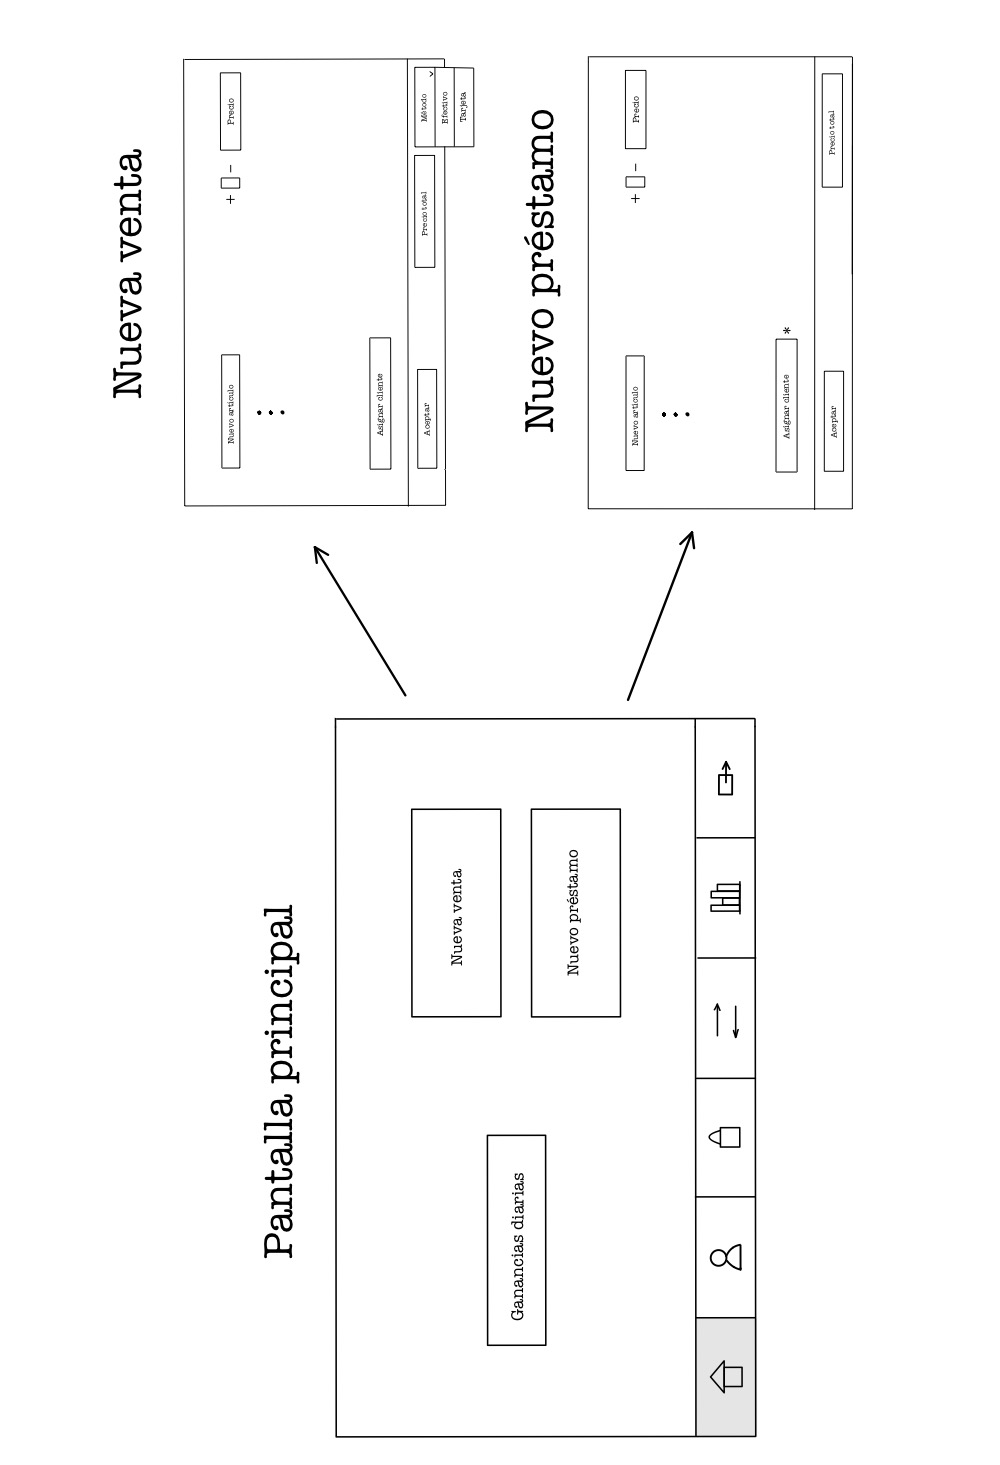
\includegraphics[width=0.8\textwidth, angle=270]{imagenes/pantalla_principal.JPG}
	\caption{Diseño de la pantalla principal.}
	\label{fig:pantallaprincipal}
\end{figure}



\subsection{Pantalla de clientes}

\begin{figure}[ht]
	\centering
	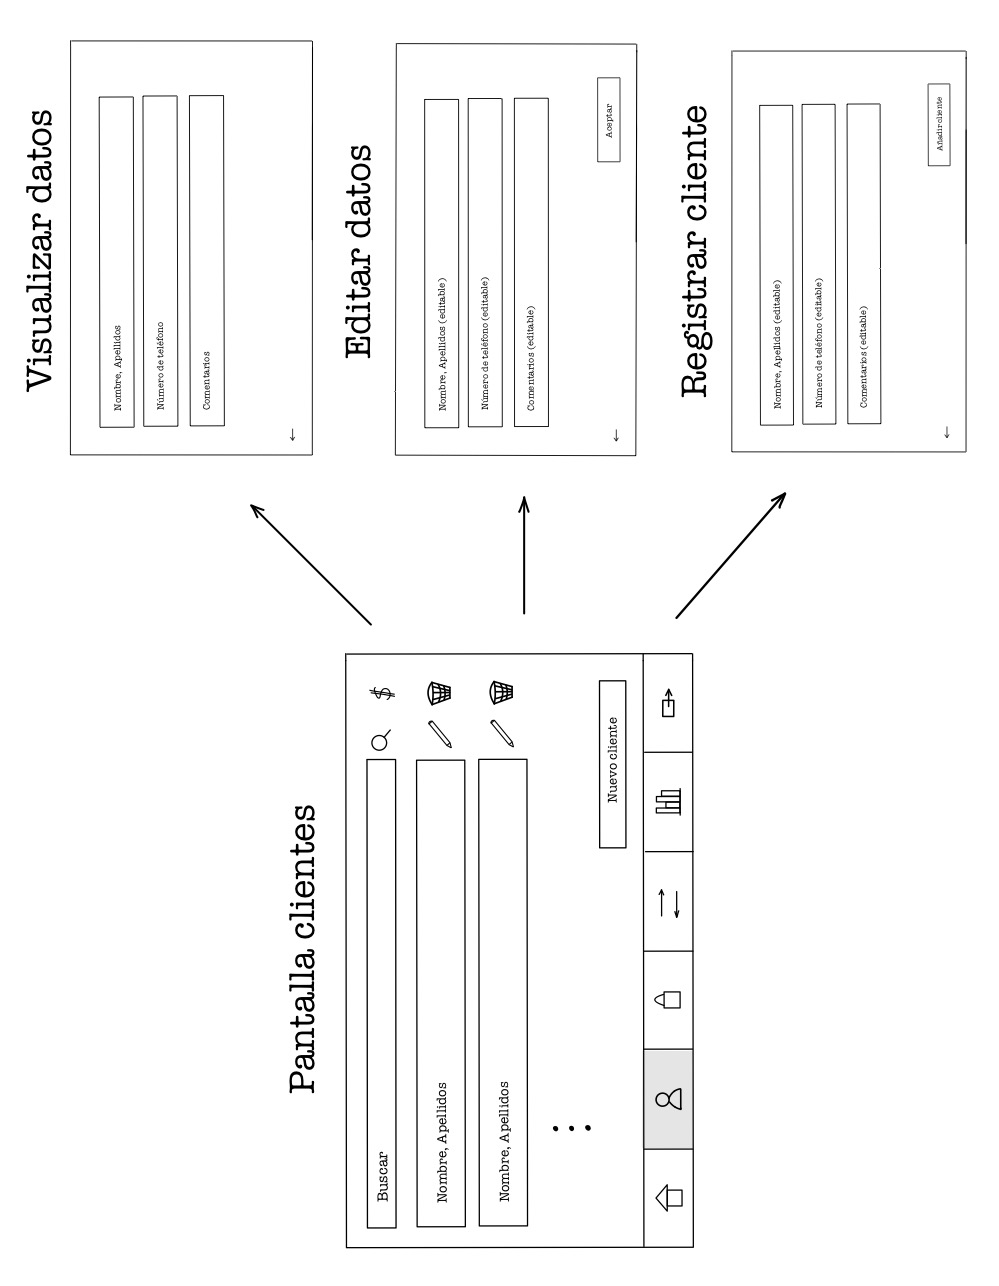
\includegraphics[width=0.8\textwidth, angle=270]{imagenes/pantalla_clientes.JPG}
	\caption{Diseño de la pantalla clientes.}
	\label{fig:pantallaclientes}
\end{figure}

\newpage

\subsection{Pantalla de artículos}

\begin{figure}[ht]
	\centering
	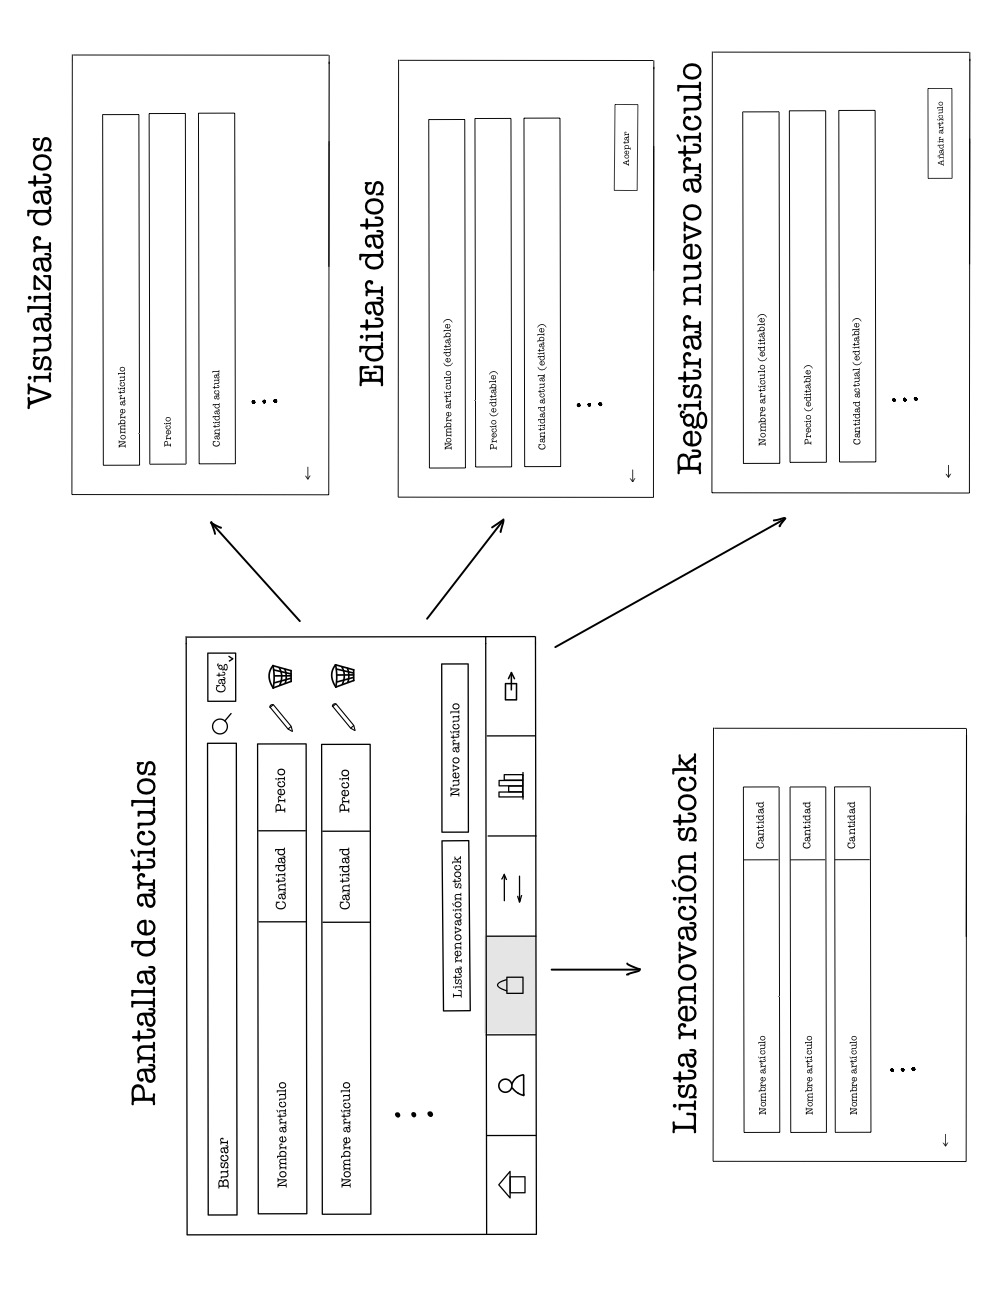
\includegraphics[width=0.8\textwidth, angle=270]{imagenes/pantalla_articulos.JPG}
	\caption{Diseño de la pantalla artículos.}
	\label{fig:pantallaarticulos}
\end{figure}

\newpage


\subsection{Pantalla de movimientos}

\begin{figure}[ht]
	\centering
	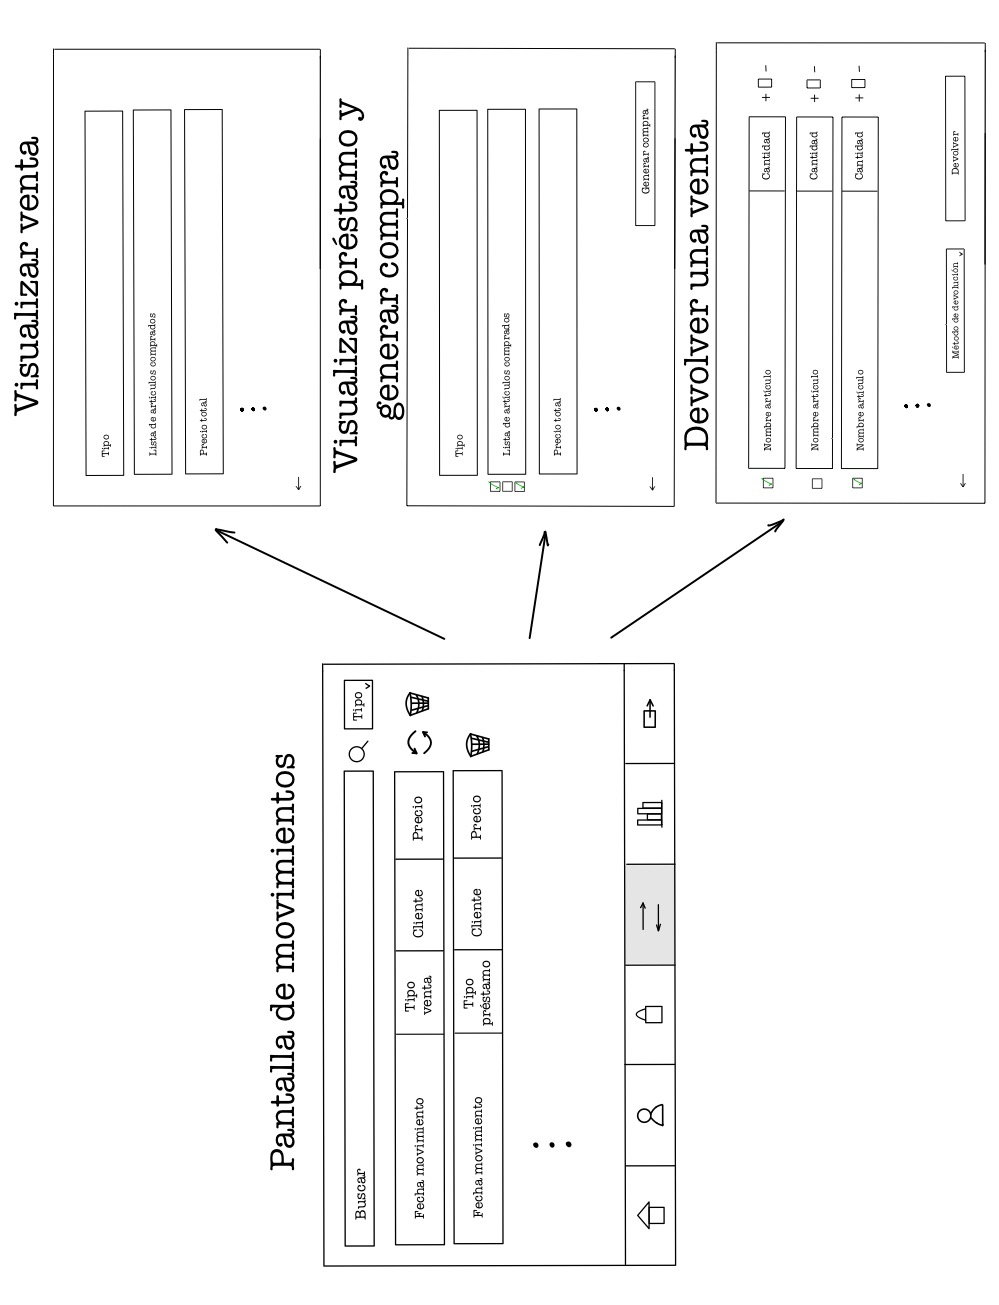
\includegraphics[width=0.8\textwidth, angle=270]{imagenes/pantalla_movimientos.JPG}
	\caption{Diseño de la pantalla movimientos.}
	\label{fig:pantallamovimientos}
\end{figure}

\newpage

\subsection{Pantalla de gráficos}

\begin{figure}[ht]
	\centering
	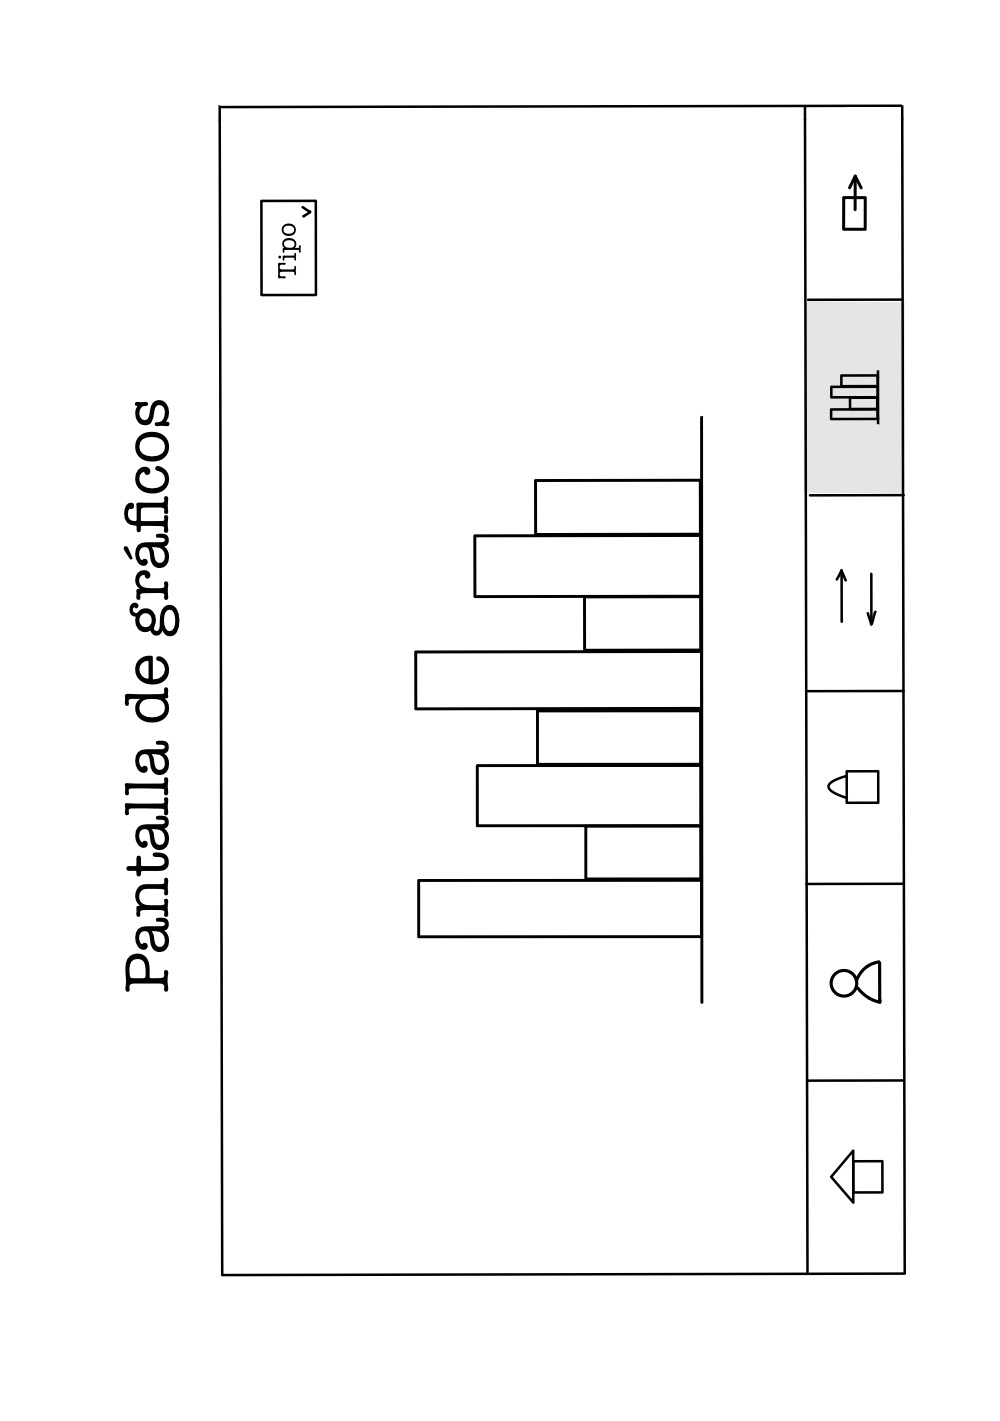
\includegraphics[width=0.8\textwidth, angle=270]{imagenes/pantalla_graficos.JPG}
	\caption{Diseño de la pantalla gráficos.}
	\label{fig:pantallagraficos}
\end{figure}
%
%\input{capitulos/06_Implementacion}
%
%\input{capitulos/07_Pruebas}
%
%\input{capitulos/08_Conclusiones}
%
%%\chapter{Conclusiones y Trabajos Futuros}
%
%
%%\nocite{*}
%\bibliography{bibliografia/bibliografia}\addcontentsline{toc}{chapter}{Bibliografía}
%\bibliographystyle{miunsrturl}
%
%\appendix
%\input{apendices/manual_usuario/manual_usuario}
%%\input{apendices/paper/paper}
%\input{glosario/entradas_glosario}
% \addcontentsline{toc}{chapter}{Glosario}
% \printglossary
%\chapter*{}
%\thispagestyle{empty}


